\documentclass[11pt,a4paper]{article}

\usepackage[T1]{fontenc}
\usepackage[utf8]{inputenc}
\usepackage{geometry}
\usepackage{graphicx}
\usepackage{booktabs}
\usepackage{array}
\usepackage{textcomp}
\usepackage[hyphens]{url}
\usepackage[numbers,sort&compress]{natbib}
\usepackage{hyperref}
\usepackage{lineno}

\geometry{margin=2.5cm}
\raggedbottom

\newcommand{\affil}[1]{\textsuperscript{#1}}
\usepackage{xr-hyper}
\externaldocument{bmsim_si}
\linenumbers

\begin{document}

\title{Bloch-McConnell Simulation Study – Comparison of Various CEST Simulation Frameworks}

\author{\parbox{\textwidth}{\centering
Markus Huemer\affil{1},
Patrick Schuenke\affil{2,3},
Viktoria Buchegger\affil{1},
Martin Juschitz\affil{1},
Nick Scholand\affil{1,4},
Felix F. Zimmermann\affil{2},
Christoph Kolbitsch\affil{2},
Moritz Simon Fabian\affil{5},
Nikita Vladimirov\affil{6},
Or Perlman\affil{6,7},
Swee Qi Pan\affil{8,9},
Yee Kai Tee\affil{8},
Ouri Cohen\affil{10},
Huabin Zhang\affil{11},
Jianpan Huang\affil{11},
Jian Hou\affil{12},
Qing Zeng\affil{13,14},
Nirbhay Yadav\affil{13,14},
Jiadi Xu\affil{13,14},
Kexin Wang\affil{13,14,15},
Beomgu Kang\affil{13,14},
Munendra Singh\affil{13,14},
Hye-Young Heo\affil{13,14},
Jingpu Wu\affil{14,16},
Jinyuan Zhou\affil{14},
Dario Livio Longo\affil{17},
Feriel Ramdhane\affil{17},
Zhongliang Zu\affil{18},
Malvika Viswanathan\affil{18},
Pedram Parnianpour\affil{19},
Erik P. Pioro\affil{19},
Mara Quach\affil{20,21},
Rudolf Stollberger\affil{1},
Martin Uecker\affil{1},
Moritz Zaiss\affil{5}
\\[1ex]
\small \affil{1}Institute of Biomedical Imaging, Graz University of Technology, Graz, Austria\\
\small \affil{2}Physikalisch-Technische Bundesanstalt (PTB), Braunschweig and Berlin, Germany\\
\small \affil{3}NVision Quantum Technologies, Ulm, Germany\\
\small \affil{4}Siemens Healthineers, Erlangen, Germany\\
\small \affil{5}Institute of Neuroradiology, Friedrich-Alexander-Universität Erlangen-Nürnberg (FAU),\\
\small University Hospital Erlangen, Erlangen, Germany\\
\small \affil{6}School of Biomedical Engineering, Tel Aviv University, Tel Aviv, Israel\\
\small \affil{7}Sagol School of Neuroscience, Tel Aviv University, Tel Aviv, Israel\\
\small \affil{8}Lee Kong Chian Faculty of Engineering and Science, Universiti Tunku Abdul Rahman, Kajang, Malaysia\\
\small \affil{9}Philips Singapore, Singapore, Singapore\\
\small \affil{10}Department of Medical Physics, Memorial Sloan Kettering Cancer Center, New York, USA\\
\small \affil{11}Department of Diagnostic Radiology, Li Ka Shing Faculty of Medicine, The University of Hong Kong, Hong Kong\\
\small \affil{12}Department of Imaging and Interventional Radiology, The Chinese University of Hong Kong, Hong Kong\\
\small \affil{13}F.M. Kirby Research Center for Functional Brain Imaging, Kennedy Krieger Institute, Baltimore, USA\\
\small \affil{14}Department of Radiology and Radiological Science, Johns Hopkins University School of Medicine, Baltimore, USA\\
\small \affil{15}Biomedical Imaging Research Institute, Cedars-Sinai Medical Center, Los Angeles, California, USA\\
\small \affil{16}Department of Electrical and Computer Engineering, Johns Hopkins University, Baltimore, USA\\
\small \affil{17}Institute of Biostructures and Bioimaging, National Research Council of Italy, Torino, Italy\\
\small \affil{18}Institute of Imaging Science, Vanderbilt University Medical Center, Nashville, USA\\
\small \affil{19}Djavad Mowafaghian Centre for Brain Health, University of British Columbia, Vancouver, Canada\\
\small \affil{20}Department of Biomedical Engineering and Graeme Clark Institute, The University of Melbourne, Parkville, Australia\\
\small \affil{21}Melbourne Brain Centre Imaging Unit, The University of Melbourne, Parkville, Australia
}}

\date{\today}

\maketitle

\begin{abstract}
\noindent\textbf{Purpose:} Quantitative chemical exchange saturation transfer (CEST) MRI depends on Bloch-McConnell simulations, yet it is unclear how consistent implementations are across research groups. This study quantified inter-framework variability and identified dominant sources of disagreement.

\noindent\textbf{Methods:} Eight benchmark cases were defined and distributed online in two rounds: four continuous-wave preparations on a two-pool creatine and a five-pool white-matter model (cases 1--4), followed by Gaussian and pulsed WASABI preparations (cases 5--8). Nineteen groups submitted $Z$-spectra for comparison.

\noindent\textbf{Results:} For simple two-pool CW saturation (cases 1--2), most submissions agreed within $\sim 10^{-4}$ in $Z$-spectra difference, but residual spread exceeded numerical precision. 
By contrast, marked differences were observed in the simulations for the five-pool model (cases 3--4) and time-dependent saturation pulses (cases 5--7). 
The different implementation of the magnetization transfer (MT) pool was identified as a major contributor to these differences. 
Overall case 5 (a single Gaussian pulse) showed the largest variability among groups; related pulse trains (cases 6--7) displayed additional sideband differences, whereas a short two-pulse WASABI scheme (case 8) agreed more closely.
The final observed differences in the simulations could lead to biases of tens of percent in the fitted pool fractions or exchange rates. 


\noindent\textbf{Conclusion:} Although the presented study helped to find common ground, Bloch-McConnell simulators from different groups are not yet interchangeable, even for fully specified protocols. Harmonized MT modeling (full $M_{xyz}$ versus $z$-only), shaped-pulse handling, and clear RF power definitions are prerequisites for reproducible quantitative CEST. This open benchmark supports ongoing validation and community standardization.
\end{abstract}

\noindent\textbf{Keywords:} CEST, MRI, Bloch-McConnell, magnetization transfer, quantitative MRI, inter-site comparison

\noindent\textbf{Correspondence:} Markus Huemer, Institute of Biomedical Imaging, Graz University of Technology, Stremayrgasse 16/III, 8010 Graz, Austria. Email: \texttt{huemer@tugraz.at}



%FIXME Or Pearlman: Moritz, do we need to replace the number "ZA 814/15-1" with "559955894"?

\noindent\textbf{Wordcount:} Abstract: \~200, Main text: \~4000


\section{Introduction}\label{introduction}

Chemical Exchange Saturation Transfer (CEST) MRI is a powerful imaging technique that provides contrast sensitive to exchange processes between solute and water protons. This sensitivity enables novel contrasts that are increasingly explored in clinical MRI applications. Among the most commonly studied CEST contrasts is amide proton transfer weighted (APTw) imaging, which has been used in various organs and has been shown to be particularly useful in the assessment of cancer \cite{Zhou2022Consens}, neurodegenerative diseases \cite{ChenLin2019}, and other pathologies like ischemic stroke \cite{Tietze2014}. In the context of cancer, CEST MRI has been used to differentiate tumor progression from radiation necrosis \cite{Zeyen2025}, assess treatment response \cite{Kroh2023}, and detect genetic mutations such as IDH in gliomas \cite{Paech2018}. Recently, there has been growing interest in quantitative CEST approaches (qCEST), which aim to provide quantitative insights into exchange rates and solute concentrations. Such approaches include Bloch-McConnell model fitting, ratiometric methods, and CEST MR fingerprinting.
Quantitative CEST analysis techniques are based on the Bloch-McConnell equations, which extend the classical Bloch equations to systems of coupled proton pools with chemical exchange \cite{McConnell1958}. For a system of $N$ pools, the magnetization vector $\mathbf{M}$ contains the transverse and longitudinal components of each pool. During RF irradiation at offset $\Delta\omega$, the time evolution is described by 
\begin{equation}
\dot{\mathbf{M}} = \mathbf{A}(\Delta\omega, B_1, \ldots)\mathbf{M} + \mathbf{c},
\label{eq:bm}
\end{equation}
where $\mathbf{A}$ encodes relaxation, chemical exchange, off-resonance effects, and RF saturation, and $\mathbf{c}$ accounts for equilibrium magnetization. By simulating this evolution for a defined saturation scheme and a range of offsets, one obtains model $Z$-spectra and derived contrasts such as magnetization transfer ratio asymmetry ($MTR_{\mathrm{asym}}$) \cite{Zhou2003}. Because qCEST fitting and fingerprinting pipelines depend directly on these forward simulations, differences between numerical implementations can translate into biases in estimated pool sizes and exchange rates.

Numerous simulation frameworks have been developed to perform Bloch-McConnell simulations, ranging from tools used exclusively within individual research groups to open-source platforms such as Pulseq-CEST \cite{Herz2021}, BMCTool \cite{SchuenkeBMC}, and CEST GUI \cite{Zhang2025}. Despite the availability of these tools, no systematic comparison between different simulation frameworks has been conducted. Because qCEST pipelines depend directly on forward simulations, differences in Bloch-McConnell implementations can propagate to differences in fitted pool parameters and exchange rates. Without a shared reference or ground truth, it remains difficult to judge whether observed variability in qCEST metrics reflects biology, acquisition, or simulation implementation, which makes cross-study comparisons challenging.

The objective of this work is to address this gap by providing a baseline to compare and ultimately validate Bloch-McConnell simulations from various CEST research groups. To achieve this, we defined two rounds of Bloch-McConnell simulation scenarios, each comprising four cases with well-defined saturation schemes and pool models. These cases were designed to capture a range of commonly encountered CEST saturation settings, including simple CW preparations, shaped-pulse trains as used on clinical MRI scanners, and pool configurations ranging from simple phantoms to brain tissue. Using this benchmark, we compared simulation results from up to 20 different groups, offering new insights into the consistency and reliability of Bloch-McConnell simulations across the field.

\section{Methods}\label{methods}

All necessary simulation settings and information were provided on the public GitHub repository at \url{https://github.com/pulseq-cest/BMsim_challenge}. The dataset used for the figures and analyses in this manuscript is archived on Zenodo at \url{https://doi.org/10.5281/zenodo.21265597}.

\subsection{General Simulation Settings}
The following settings applied to all benchmark cases unless stated otherwise.
\begin{itemize}
    \item Fully relaxed initial longitudinal magnetization ($Z_i = 1$) before simulating each offset. Equivalently, the recovery interval between offsets must satisfy $T_{\mathrm{rec}} > 10 \cdot T_1$ of the slowest pool (e.g.\ water with $T_1=3$~s in the 2-pool model requires $T_{\mathrm{rec}} > 30$~s). All pool-model YAML files specify \texttt{reset\_init\_mag: True} for this purpose. The shorter recovery delays $T_{\mathrm{rec}}=3.5$~s (cases 1--3, 5--7) or $3$~s (case 4) in the reference Pulseq files are \emph{not} part of the simulation specification; they reflect typical scanner timing between acquisitions and must not be used as a substitute for resetting $Z_i=1$.
    \item Relative concentration of water is set to one ($f_{water}=1$)
    \item After each saturation a delay of $6.5$~ms was simulated to account for the spoiler gradient, which would normally be applied in measurements (post-preparation delay $t_{\mathrm{delay}} = 6.5$~ms).
    \item Gyromagnetic ratio: $42.5764$~MHz/T, which leads to a Larmor frequency (for $3$~T) of $127.7292$~MHz
    \item Normalization scan at $-300$~ppm using the same preparation
\end{itemize}

\subsection{Pool Models}\label{pool_models}
Two different pool models were defined and used in the eight simulation cases. The first pool model is a 2-pool model and consists of a water and one single guanidine-like CEST pool. It is supposed to mimic the situation in a creatine phantom. 
The second pool model is a 5-pool model consisting of a water pool, an ssMT pool, an amide-like CEST pool, a guanidine-like CEST pool and a rNOE pool, in order to mimic more complex in vivo like environments.
The pool model configuration files were defined in human- and machine readable yaml file format and can be found in the GitHub repository as well as in Supporting Information Section~\ref{si:poolmodels}.


\begin{figure}[t]
\centering
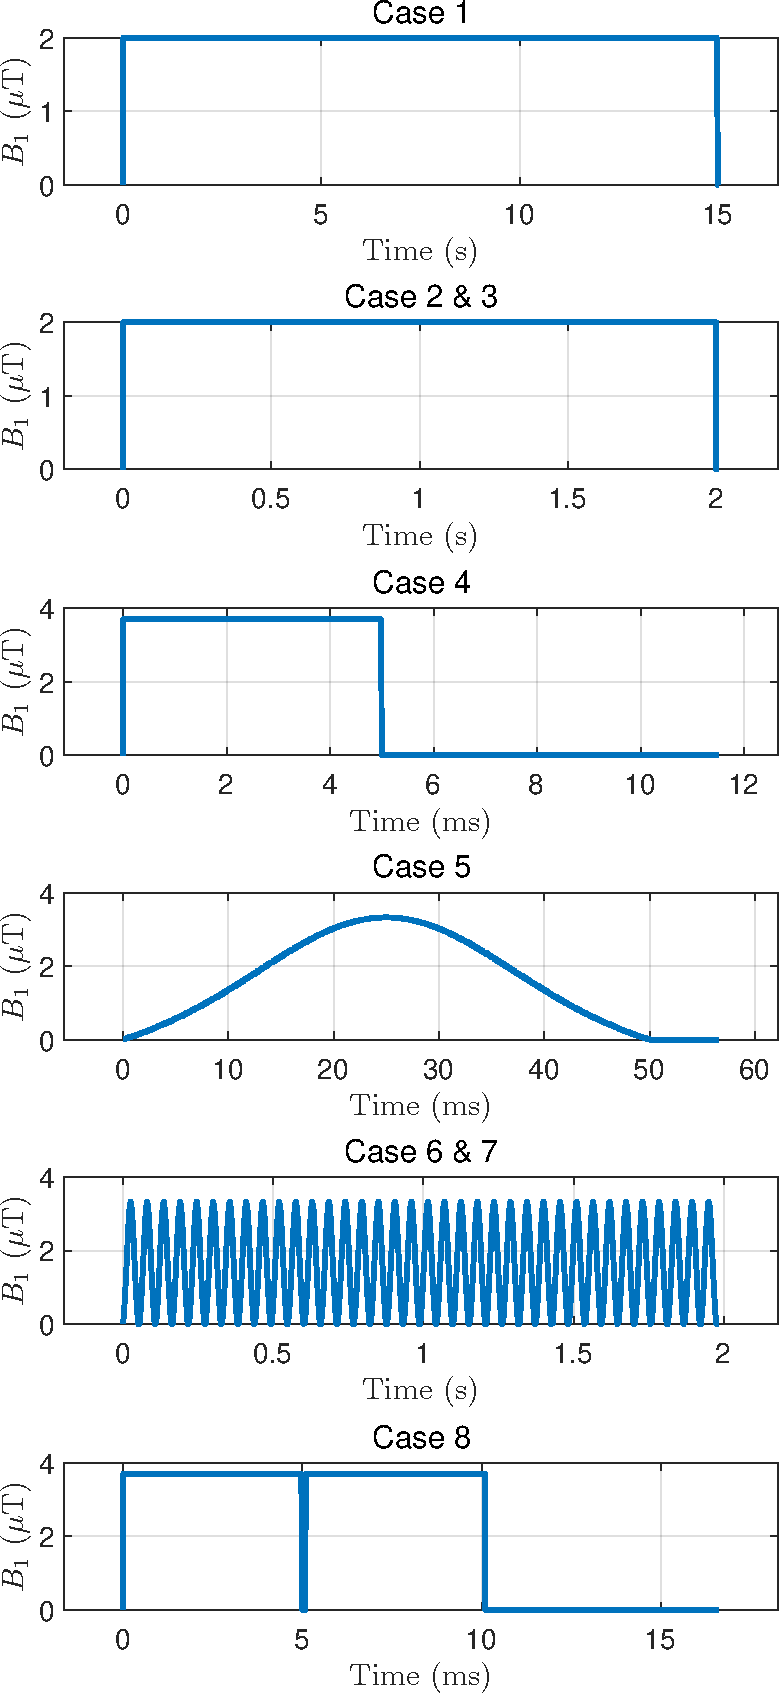
\includegraphics[width=0.9\linewidth,height=0.8\textheight,keepaspectratio]{figures/Pulses.pdf}
\caption{Saturation types for all tested cases. Cases 1 to 4 use CW saturation with different saturation times. Cases 5, 6 and 7 use one or multiple Gaussian pulses and Case 8 repeats the CW saturation of Case 4 with a short interpulse delay. Note the spoiler delay after the pulses visible for short saturation cases.  }
\label{fig:Pules}
\end{figure}

\subsection{Simulation Cases}
In total, eight cases of increasing complexity were compared in two rounds on the pool models described in Section \ref{pool_models}. An overview with the parameters for all cases is listed in Table \ref{table_sim_cases} and the saturation pulses are shown in Figure \ref{fig:Pules}.


\subsubsection{Round 1}


In the first round of the challenge, four cases with continuous-wave (CW) saturation and different saturation times were tested. The aim was to cover cases that should first be comparatively straightforward to reproduce and then add complexity from shorter saturation times, additional exchanging pools, and MT modeling afterwards.
\begin{itemize}
\item \textbf{Case 1:} A $15$~s CW saturation on the 2-pool model with $B_{1}=2\,\mu T$. This case tests the steady-state for a simple creatine-like phantom and was intended as a baseline test for exchange, relaxation, offset handling, and sign conventions.
\item \textbf{Case 2:} A $2$~s CW saturation on the same 2-pool model with $B_{1}=2\,\mu T$. Compared with Case 1, this case emphasizes transient saturation behavior while keeping the pool model unchanged, thereby testing whether implementations agree away from the full steady-state.
\item \textbf{Case 3:} The same $2$~s CW saturation as in Case 2, but applied to the 5-pool white-matter model. This case tests the handling of multiple exchanging pools and, in particular, the implementation of the semisolid MT pool.
\item \textbf{Case 4:} A short block-pulse preparation as used in the WASABI method \cite{Schuenke2017}, consisting of a $5$~ms pulse with $B_{1}=3.7\,\mu T$ applied to the 5-pool white-matter model. This case probes short-pulse and off-resonance behavior in a multi-pool system, including the influence of MT and phase evolution during a brief RF event.
\end{itemize}


\subsubsection{Round 2}
In the second round, pulsed saturation using Gaussian and block-pulse preparations was compared on the same models. These cases were designed to test whether groups implemented shaped RF pulses, interpulse delays, and pulse trains consistently when the saturation preparation is provided in a machine-readable format.
\begin{itemize}
\item \textbf{Case 5:} A single Gaussian pulse with $t_p=50$~ms and $B_{1,\mathrm{rms}}=1.9962\,\mu T$ on the 2-pool model. The pulse shape was provided as a CSV file with time and amplitude values. This isolated pulse tests interpolation, pulse handling and RF amplitude scaling, without additional complications from a pulse train.
\item \textbf{Case 6:} The Gaussian pulse from Case 5 repeated 36 times with an interpulse delay $t_d=5$~ms, for a combined $T_{sat}$ of 1.975~s, again on the 2-pool model. This case extends Case 5 to a clinically relevant pulse train and tests accumulation of saturation and relaxation over repeated RF events.
\item  \textbf{Case 7:} The same Gaussian pulse train as in Case 6, but applied to the 5-pool white-matter model. This case combines shaped-pulse train implementation with the multi-pool and MT-modeling complexity introduced in Case 3.
\item  \textbf{Case 8:} The WASABI pulse from Case 4 ($B_{1}=3.7\,\mu T$) played out twice with an interpulse delay $t_d=100\,\mu s$ on the 5-pool white-matter model. This short two-pulse preparation tests whether implementations handle phase accumulation and relaxation during very short delays consistently.
\end{itemize}





\begin{table}[t]%
\centering
\caption{Overview over the different simulation cases. CW block pulses (cases 1--4) use constant $B_1$ amplitude; WASABI block pulses (cases 4 and 8) use $B_{1,\mathrm{peak}}$; Gaussian pulses (cases 5--7) use $B_{1,\mathrm{rms}}$.}\label{table_sim_cases}
\begin{tabular*}{\textwidth}{@{\extracolsep\fill} >{\centering\arraybackslash}p{.5cm} >{\centering\arraybackslash}p{1.5cm} >{\centering\arraybackslash}p{1.0cm} >{\centering\arraybackslash}p{2cm} >{\centering\arraybackslash}p{2cm} >{\centering\arraybackslash}p{2cm} >{\centering\arraybackslash}p{2cm} >{\centering\arraybackslash}p{2.5cm}@{\extracolsep\fill}}
\toprule
\textbf{Case \#} & \textbf{Pool model} & \textbf{\# Pulses} & \textbf{Pulse shape}  & \textbf{Pulse duration} & \textbf{Interpulse delay} & \textbf{$B_1$} & \textbf{Offsets}  \\
\midrule
1 & 2-pool & 1 & block & 15~s & - & 2~µT & -15:0.1:15~ppm\\
2 & 2-pool & 1 & block & 2~s & - & 2~µT & -15:0.1:15~ppm\\
3 & 5-pool & 1 & block & 2~s & - & 2~µT & -15:0.1:15~ppm\\
4 & 5-pool & 1 & block & 5~ms & - & 3.7~µT & -2:0.05:2~ppm\\
5 & 2-pool & 1 & Gaussian & 50~ms & - & 1.996~µT (rms) & -2:0.02:2~ppm\\
6 & 2-pool & 36 & Gaussian & 50~ms & 5~ms & 1.996~µT (rms) & -15:0.1:15~ppm\\
7 & 5-pool & 36 & Gaussian & 50~ms & 5~ms & 1.996~µT (rms) & -15:0.1:15~ppm\\
8 & 5-pool & 2 & block & 5~ms & 100~µs & 3.7~µT & -2:0.05:2~ppm\\
\bottomrule
\end{tabular*}
\end{table}





\subsection{Entries and participating groups}
In total, 20 groups or solver teams participated in the study. Some groups submitted multiple solver variants or additional z-only MT simulations. Additionally, some groups did not submit results for all cases, leading to the following number of submitted entries per case:
\begin{itemize}
\item \textbf{Case 1:} 22 entries
\item \textbf{Case 2:} 23 entries
\item \textbf{Case 3:} 24 entries
\item \textbf{Case 4:} 23 entries
\item \textbf{Case 5:} 18 entries
\item \textbf{Case 6:} 19 entries
\item \textbf{Case 7:} 19 entries
\item \textbf{Case 8:} 19 entries
\end{itemize}
Additional information on the participating groups, solver variants, and implementation details is provided in Table~\ref{tab:participants} and Supporting Information Section~\ref{si:simulations}.

The main comparison figures exclude entries labeled as z-only MT simulations, except for the dedicated $M_{xyz}$ versus $z$-only MT comparison in Section~\ref{subsec:res:zMT}.


\begin{table}[htbp]
\centering
\caption{Overview of participating groups, solver variants, and implementation details. Submission numbers are used as labels in the comparison figures and were assigned in the order of submission.}
\label{tab:participants}
\resizebox{\textwidth}{!}{%
\begin{tabular}{clccccc}
\textbf{Subm.} & \textbf{Corresponding Participant} & \textbf{Prog. Language} & \textbf{Number of Pools} & \textbf{MT} & \textbf{Solver} & \textbf{Paper \& Code} \\ \hline
S01 & \textbf{Moritz Zaiss - FAU} & Matlab 2017b / C++ & dynamic & x,y,z & expm with Pade (6 iterations) & pulseq-cest matlab \\
S02 & \textbf{Patrick Schuenke - PTB} & python & dynamic & x,y,z & expm with eig & BMCTool - \url{github.com/schuenke/BMCTool} \\
S03 & \textbf{Markus Huemer - IBI TUG} & Matlab & 5 fixed & x,y,z & expm with Operator Splitting & \url{gitlab.tugraz.at/ibi/mrirecon/miscellaneous/bmc-simulation-matlab}\cite{Graf2021} \\
S04 & \textbf{Markus Huemer - IBI TUG} & Matlab & 7 fixed & x,y,z & expm with eig &  \\
S05 & \textbf{Qing Zeng - KKI/JHU} & Python & dynamic & x,y,z & expm &  \\
S06 & \textbf{Nikita Vladimirov - TAU} & Python/C++ & dynamic & x,y,z & Pade & \begin{tabular}{@{}c@{}}open-py-cest-mrf \cite{Vladimirov2025} \\ \url{github.com/momentum-laboratory/molecular-mrf}\end{tabular}  \\
S07 & \textbf{Zhongliang Zu - VUMC} & Matlab & dynamic & only z & expm with eig &  \\
S08 & \textbf{Kexin Wang - KKI/JHU} & Matlab & fixed & x,y,z & expm &  \url{github.com/Kexin-Wang/BMsim}\cite{Wang2024}\\
S09 & \textbf{Dario Longo - CNR} & Matlab 2021b & fixed & x,y,z & expm & extension of \url{github.com/cest-sources/BM_sim_fit}\cite{Zaiss2018}
 \\
S10 & \textbf{Moritz Fabian - FAU} & Matlab 2019b/2022b & dynamic & x,y,z & RKDP & \url{gitlab.com/mrilab/sim/bmsim.git} \\
S11 & \textbf{Beomgu Kang - KKI/JHU} & Matlab / python & dynamic & x,y,z & expm & \url{github.com/Heo-Group}\cite{Singh2023} \\
S12 & \textbf{Huabin Zhang - HKU} & Matlab 2023a & dynamic & x,y,z & expm & \url{ github.com/JianpanHuang/BMsim_challenge} \\
S13 & \textbf{Jian Hou - CUHK} & Matlab 2023a & dynamic & only z & expm &  \\
S14 & \textbf{Viktoria Buchegger - IBI TUG} & C & fixed & x,y,z & RKDP &  \begin{tabular}{@{}c@{}}BART \cite{Scholand2023} \\ \url{codeberg.org/mrirecon/bart}\end{tabular}\\
S15 & \textbf{Mara Quach - UniMelb} & Julia v1.11 & dynamic & x,y,z & Rosenbrock & \url{github.com/maraquach/CESTSim.jl}  \\ 
S16 & \textbf{Felix F. Zimmermann - PTB} & python (torch) & dynamic & x,y,z & expm & \url{github.com/fzimmermann89/mr2} \\
S17 & \textbf{Ouri Cohen - MSK} & pytorch & dynamic & x,y,z & expm &  \\
S18 & \textbf{Jingpu Wu - JHU} & python & dynamic & x,y,z & expm & \url{github.com/JimmyWu990110/BMsim_challenge_Jingpu} \\
S19 & \textbf{Pedram Parnianpour - UBC} & python & dynamic & x,y,z & expm & \url{github.com/Pedram-Parnianpour/bmsim-challenge-solver.git} \\
S20 & \textbf{Swee Qi Pan - UTAR} & Matlab & dynamic & x,y,z & expm & \url{github.com/sweeqipan/BMsim_SQPan_YKTee} \\
\hline
\end{tabular}%
}
\end{table}


\subsection{Magnetization transfer pool formulation}\label{subsec:methods:mt}
In Bloch–McConnell simulations of magnetization transfer (MT), the semisolid pool is often modeled using only longitudinal ($Z$) magnetization, assuming that transverse components decay instantaneously due to extremely short $T_2$ values. This yields a simplified scalar description in which RF irradiation affects the pool through saturation governed by an effective absorption lineshape and is also known as the Henkelmann model \cite{Graham1997}.
In contrast, a full $M_{xyz}$ formulation explicitly includes transverse components, enabling the modeling of coherent effects such as off-resonance excitation and phase evolution. The $z$-only approach is computationally efficient and frequently used in simulations for MT and also CEST experiments.
In the original formulation of this study, the way to simulate the MT pool was not explicitly stated, but results of the first round showed significant differences between $M_{xyz}$ and $z$-only MT models for the same parameters. An example of this is shown in Section~\ref{subsec:res:zMT}. 
These differences prompted a switch in the study to explicitly require $M_{xyz}$ simulations.
The zMT simulations are kept in the data source, but are not shown for all results. 
All submitted zMT only entries reported using a Lorentzian lineshape for the MT pool.


\subsection{Data analysis}\label{subsec:analysis}
Magnetization transfer ratio asymmetry ($MTR_{\mathrm{asym}}$) was computed from each $Z$-spectrum as $Z(-\Delta\omega) - Z(+\Delta\omega)$ for positive offsets $\Delta\omega$. 
Inter-submission spread was quantified point-wise at each offset as the absolute difference between the maximum and minimum value across included submissions, separately for the spectra and $MTR_{\mathrm{asym}}$; for each case we report the maximum and median spread across offsets.
The normalization measurement at $-300$~ppm was excluded from $Z$-spectrum spread calculations. 
In the main comparison figures, spectra and asymmetry curves are also shown as differences to submission S02 (BMCTool), which was used as a documented Pulseq-based reference implementation. It generally lies close to the main cluster of submissions in terms of the point-wise $Z$-spectrum spread, although it is not the median submission for every case.

\subsection{Numerical implementation checks}\label{subsec:methods:numchecks}
Two additional analyses were performed to illustrate how numerical settings can affect CEST simulations. For the BART submission (S14), single- and double-precision variants were compared with the reference S02 in Case~1 and Case~2 (Figure~\ref{fig:BARTprecision}). For the operator-splitting MATLAB submission S03, Case~7 $Z$-spectra were calculated using multiple fixed timesteps from 500 to 5~$\mu$s (Figure~\ref{fig:Case7timestep}).


\section{Results}\label{Results}
The results of the study were collected 
online at: \url{https://docs.google.com/spreadsheets/d/1JN7VN-f1ktDrJgokb0FlUFwkH0MWYlPA_jSfnQoFOVc/} and are archived here: \url{https://doi.org/10.5281/zenodo.21265597}. A simple evaluation script is available at \url{https://colab.research.google.com/drive/1csiIjK-fiftdb7OwvJ84gWuv8lLADgv7}.

\begin{figure}[!ht]
\centering
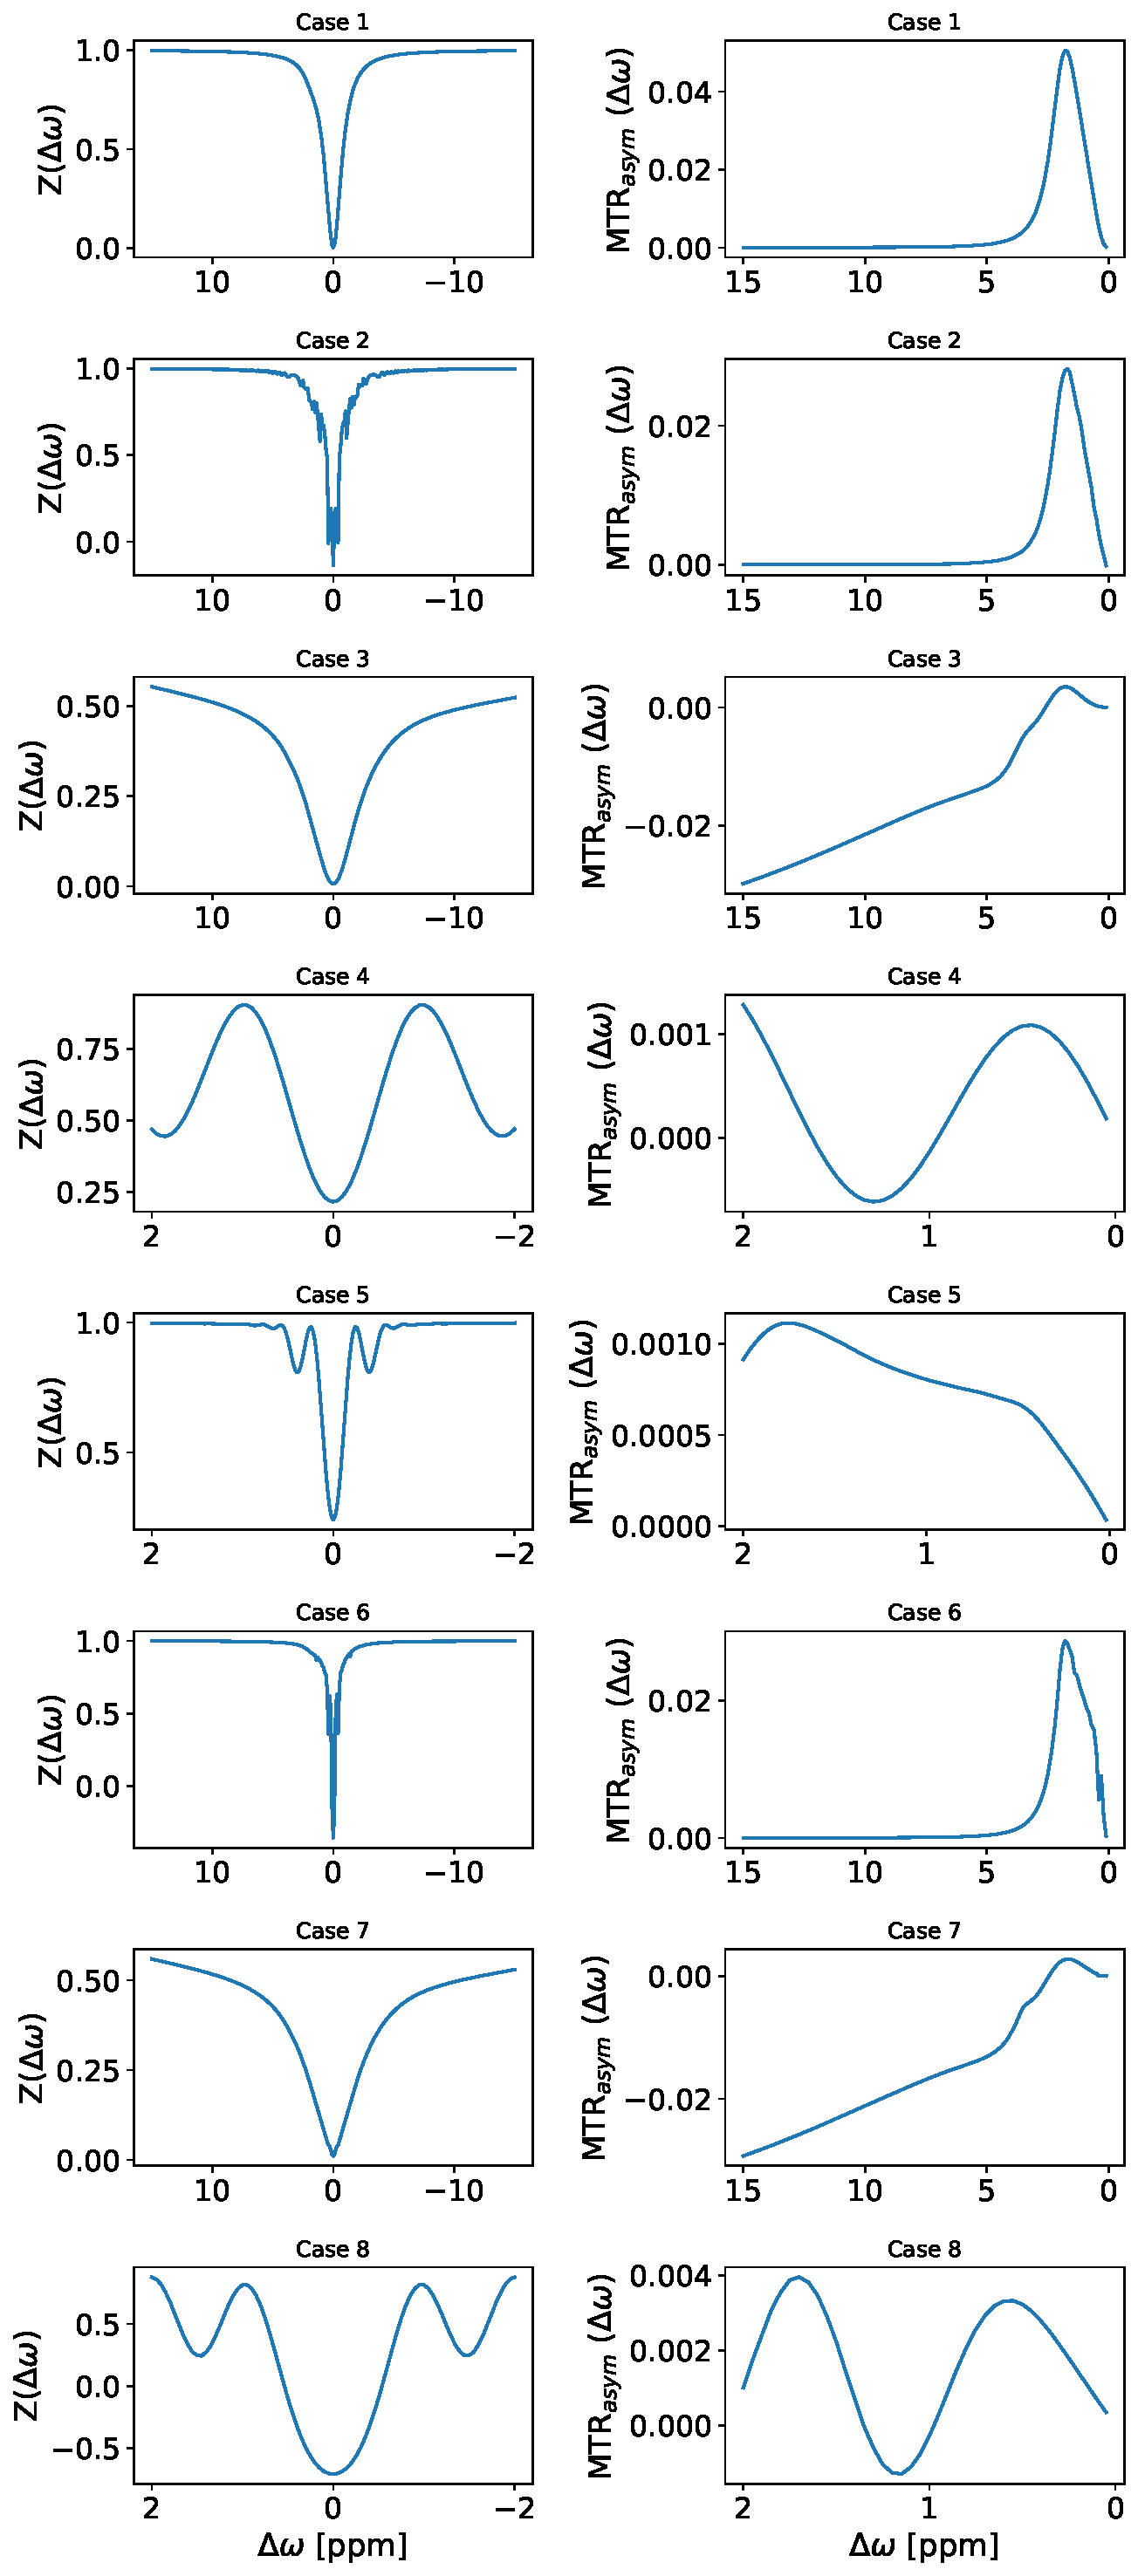
\includegraphics[width=1\linewidth,height=0.9\textheight,keepaspectratio]{figures/All_Cases_Z_and_MTRasym_ref.pdf}
\caption{Exemplary z-spectra and $MTR_{asym}$ for all eight tested cases, simulated with the MATLAB pulseq-cest implementation.}
\label{fig:RefResultsAllCases}
\end{figure}

\subsection{Round 1 results}
All results for Cases 1 and 2 are shown in Figure \ref{fig:ReasulsAll12}. Case 1 showed the closest agreement among the Round 1 scenarios. After excluding the normalization offset, the maximum spread across the submitted Z-spectra was $2.7 \times 10^{-3}$, while the median point-wise Z spread was $5.4 \times 10^{-5}$. The corresponding maximum and median $MTR_{\mathrm{asym}}$ spreads were $8.4 \times 10^{-5}$ and $9.4 \times 10^{-6}$, respectively.

For Case 2, the shorter saturation time increased the sensitivity to implementation details. Most submissions followed the same overall Z-spectrum shape, but one or more traces deviated visibly over parts of the offset range, resulting in a maximum point-wise Z spread of 0.43 and a median Z spread of $4.0 \times 10^{-3}$. The maximum and median $MTR_{\mathrm{asym}}$ spreads were 0.0095 and $3.8 \times 10^{-5}$, respectively.

All results for Cases 3 and 4 are shown in Figure \ref{fig:ReasulsAll34}. Introducing the 5-pool white-matter model in Case 3 led to broader, but more consistent deviations around the offsets affected by the CEST and MT pools. The maximum and median Z spreads were 0.031 and 0.027, and the maximum and median $MTR_{\mathrm{asym}}$ spreads were $6.5 \times 10^{-4}$ and $2.7 \times 10^{-4}$, respectively. Case 4, which used a short WASABI-like block pulse on the same pool model, showed visible differences in the Z-spectra, with maximum and median Z spreads of 0.018 and $6.9 \times 10^{-3}$, and maximum and median $MTR_{\mathrm{asym}}$ spreads of 0.0016 and $7.3 \times 10^{-4}$, respectively.

\subsection{Magnetization transfer pool formulation results}\label{subsec:res:zMT}
Selected entries are shown for Case 3 to highlight the difference between full $M_{xyz}$ MT simulations and $z$-only MT simulations in Figure \ref{fig:ReasultszMT3}. The $z$-only MT simulations formed a distinct response compared with the full $M_{xyz}$ MT implementations, especially in spectral regions where the semisolid pool contributes strongly. 
Previous analysis \cite{Schuenke2023} showed that the difference between $z$-only and $M_{xyz}$ MT simulations can lead to significant differences in fitted pool fractions and exchange rates, which can be as high as 30\% for the semisolid pool fraction or 50\% for the exchange rate.

Because this difference reflects a modeling choice rather than only a numerical solver difference, z-only MT entries were excluded from the main comparison figures. 



\subsection{Round 2 results}
All results for Cases 5 and 6 are shown in Figure \ref{fig:ReasulsAll56}. Case 5, the single Gaussian pulse, produced the largest absolute Z-spectrum spread of all cases. Although many submissions agreed closely near the central part of the spectrum, one or more submissions showed pronounced deviations, leading to a maximum Z spread of 1.45 and a median Z spread of $6.3 \times 10^{-3}$. The $MTR_{\mathrm{asym}}$ spread was much smaller, with maximum and median values of 0.0026 and $9.1 \times 10^{-4}$, respectively, because the largest spectrum deviations were largely symmetric.

In Case 6, where the same Gaussian pulse was repeated as a pulse train, the deviations persisted but changed in spectral distribution. The maximum and median Z spreads were 0.76 and $7.6 \times 10^{-3}$, and the maximum and median $MTR_{\mathrm{asym}}$ spreads were 0.0089 and $6.8 \times 10^{-5}$, respectively. The repeated pulses produced additional sideband features in the Z-spectra, which were reproduced with varying accuracy across submissions, hinting at differences in pulse train implementation, interpulse delay handling, and phase evolution during the delays.

All results for Cases 7 and 8 are shown in Figure \ref{fig:ReasulsAll78}. Case 7 combined the Gaussian pulse train with the 5-pool model and showed maximum and median Z spreads of 0.031 and $7.2 \times 10^{-3}$, and maximum and median $MTR_{\mathrm{asym}}$ spreads of $9.0 \times 10^{-4}$ and $6.9 \times 10^{-4}$, respectively. Compared with Case 6, the multi-pool model shows much closer agreement.

Case 8 showed a different pattern. The short two-pulse WASABI-like preparation produced visible Z-spectrum differences, with maximum and median Z spreads of 0.093 and 0.048. The $MTR_{\mathrm{asym}}$ curves showed maximum and median spreads of approximately $10^{-3}$ and $4.7 \times 10^{-4}$, respectively. 

\subsection{Numerical precision and time-step convergence}\label{subsec:res:numchecks}
The BART comparison in Figure~\ref{fig:BARTprecision} shows that single- and double-precision arithmetic can produce visibly different spectra, even when the underlying solver and pool model are identical. The clearest example was Case~2 ($2$~s CW saturation on the 2-pool model), where single-precision BART showed high-frequency oscillatory noise in the difference plots. The maximum point-wise deviation from S02 was approximately $1.1 \times 10^{-3}$ in $Z$ for single precision and $2.6 \times 10^{-4}$ for double precision, corresponding to an approximately fourfold reduction in peak numerical error. The mean point-wise deviation was reduced from $5.6 \times 10^{-4}$ to $3.2 \times 10^{-5}$. Case~1 ($15$~s CW saturation) showed the same pattern at smaller amplitude.


Figure~\ref{fig:Case7timestep} shows the corresponding fixed-timestep analysis for submission S03 in Case~7. A timestep of 500~$\mu$s produced a clearly different $Z$-spectrum, reducing the timestep to 100~$\mu$s produces a normal looking spectrum, which still deviates from the finest timestep of 5~$\mu$s by over 10\%. Halfing the timestep to 50~$\mu$s produces a spectrum reduces the deviation to less than 5\% and further reducing the timestep to 10~$\mu$s produces a spectrum that is indistinguishable (at the shown scale) from the finest timestep.




\begin{figure}[t]
\centering
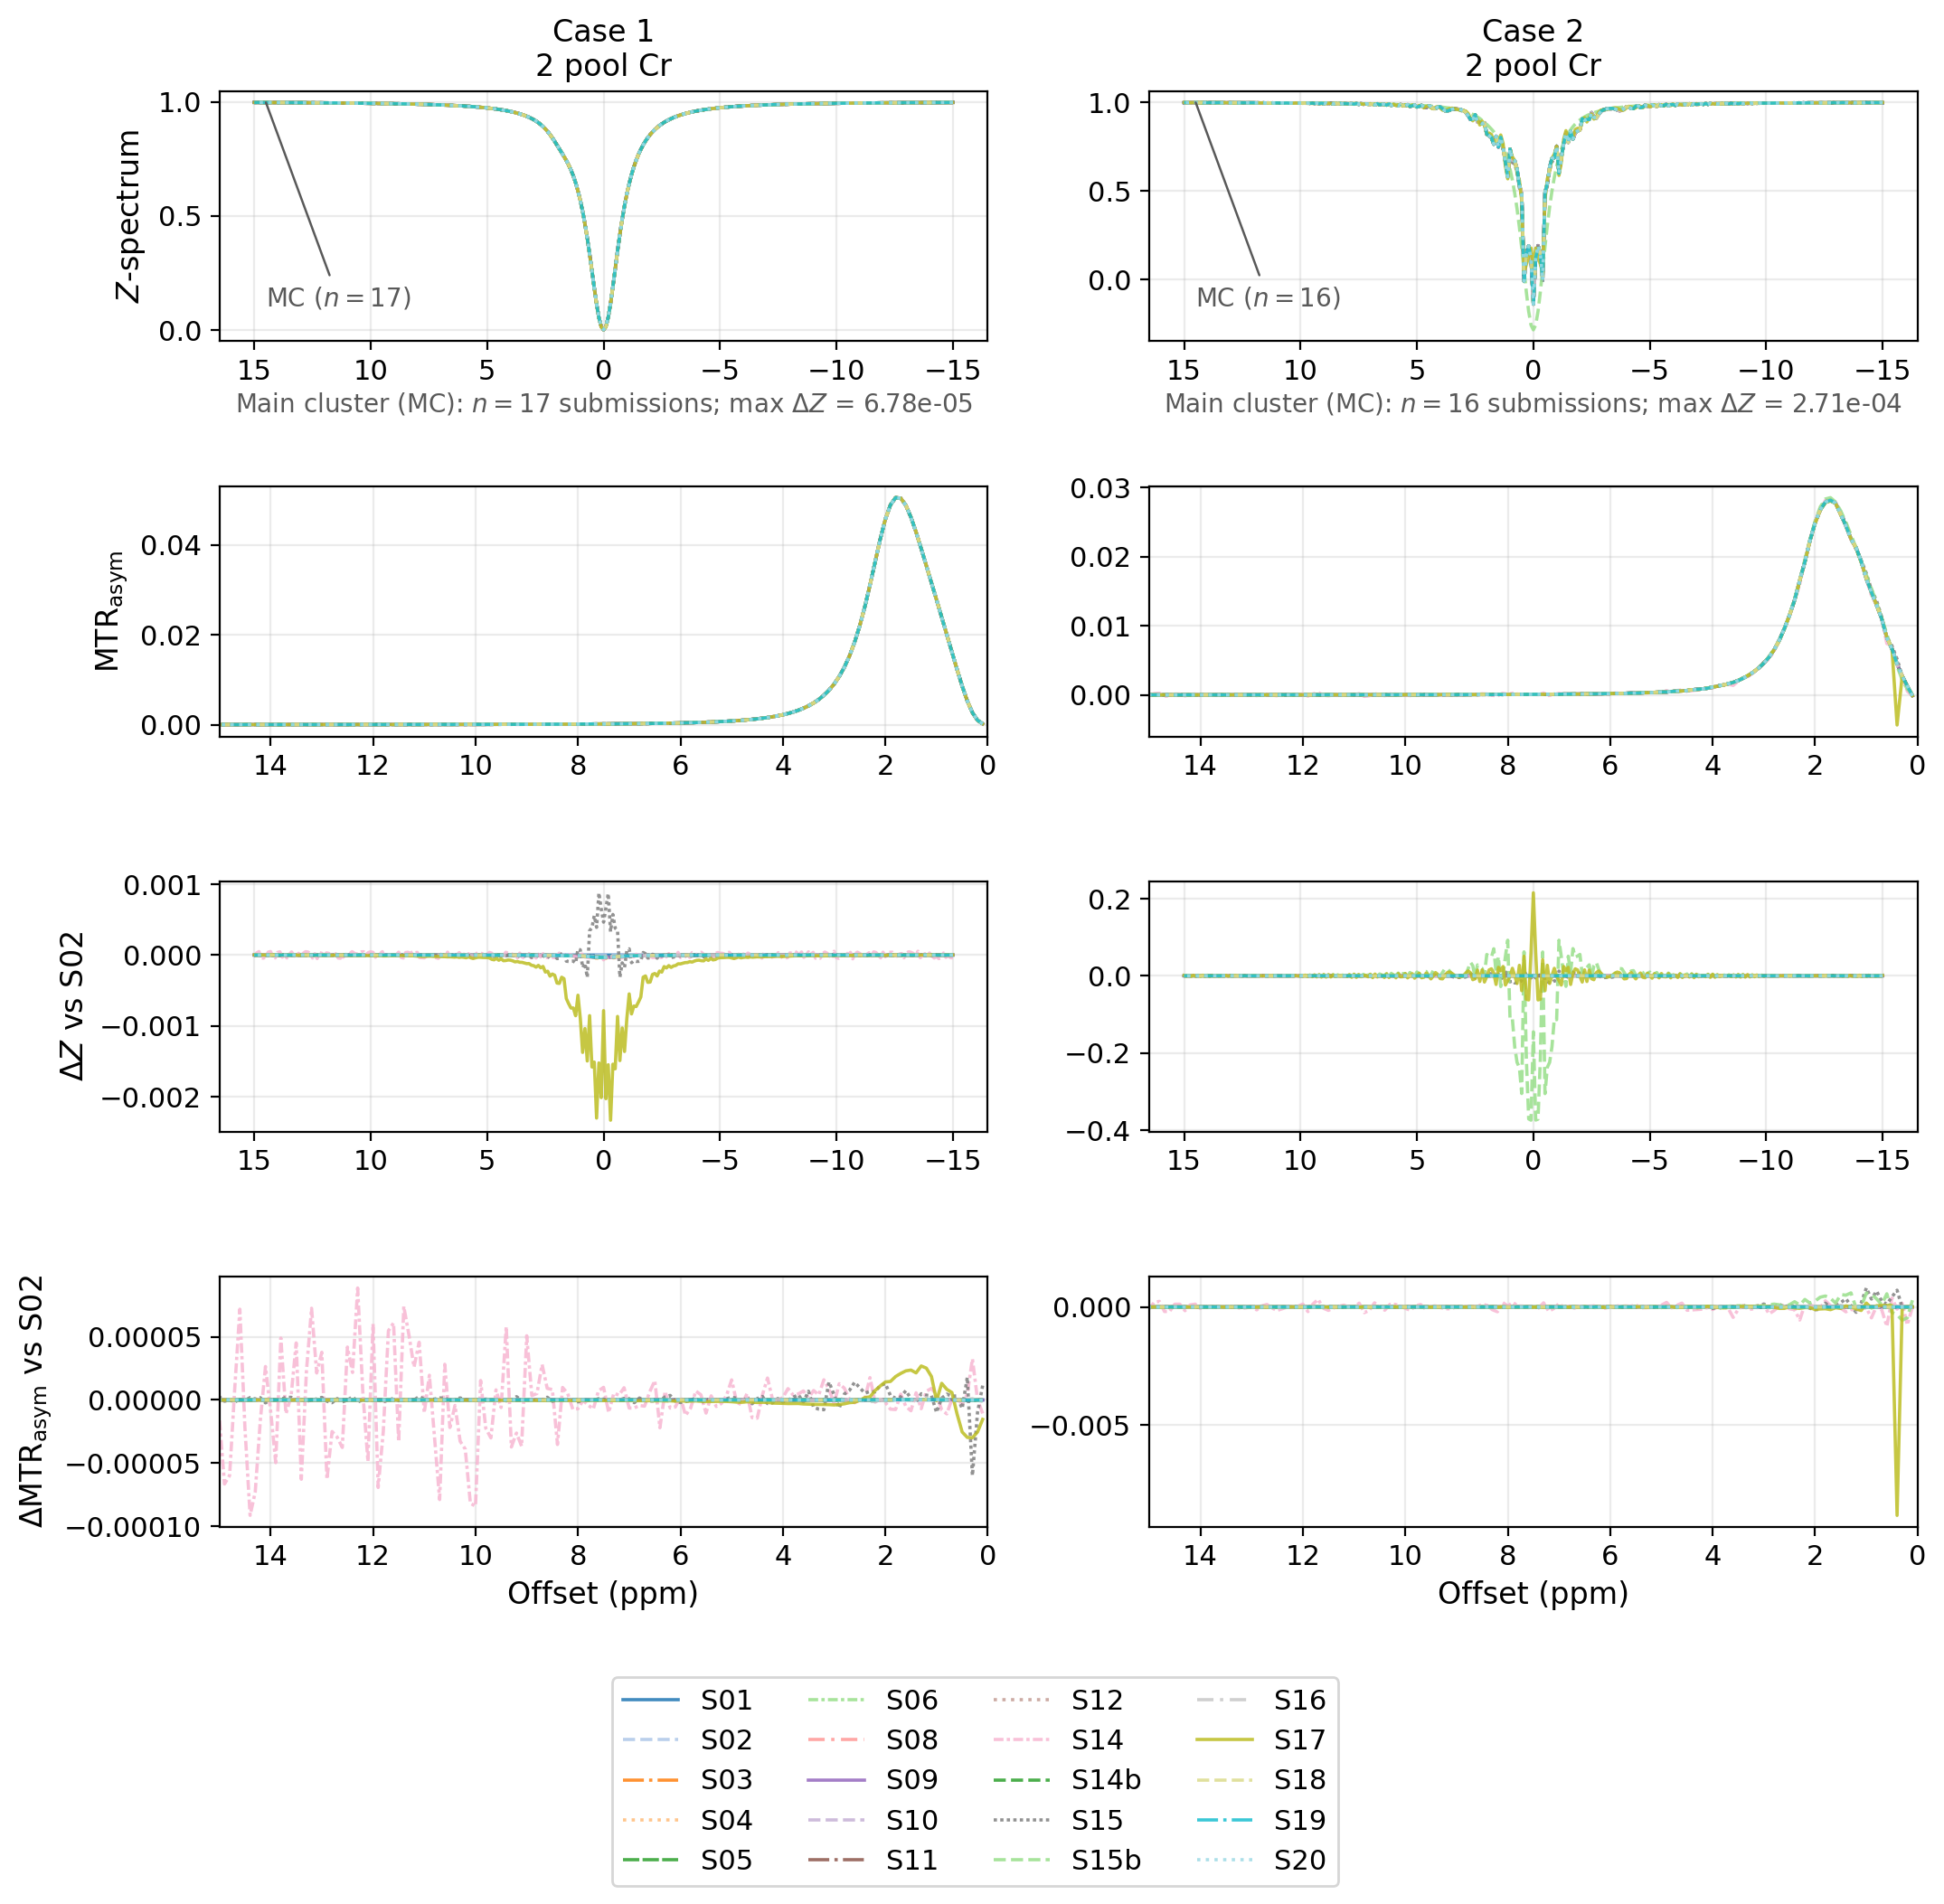
\includegraphics[width=1\linewidth]{figures/Figure_CASE_12.png}
\caption{Cases 1 and 2: $Z$- and $MTR_{asym}$ spectra with differences to S02. 
The main cluster is marked in the Z-spectra plots and contained 17 (of 19) entries in Case 1 and 16 (of 20) entries in Case 2, with maximum deviations of $6.78\cdot10^{-05}$ and $2.71\cdot10^{-04}$, respectively within those clusters.
S15 and S17 show the largest deviations in Case 1. 
S14b represents a solver variant of S14, using double precision instead of single precision. 
In Case~2, S15b denotes an alternative solver variant of S15, which shows the largest deviation from the main cluster. More information on these solver variants can be found in Supporting Information Section~\ref{si:simulations}.}
\label{fig:ReasulsAll12}
\end{figure}

\begin{figure}[t]
\centering
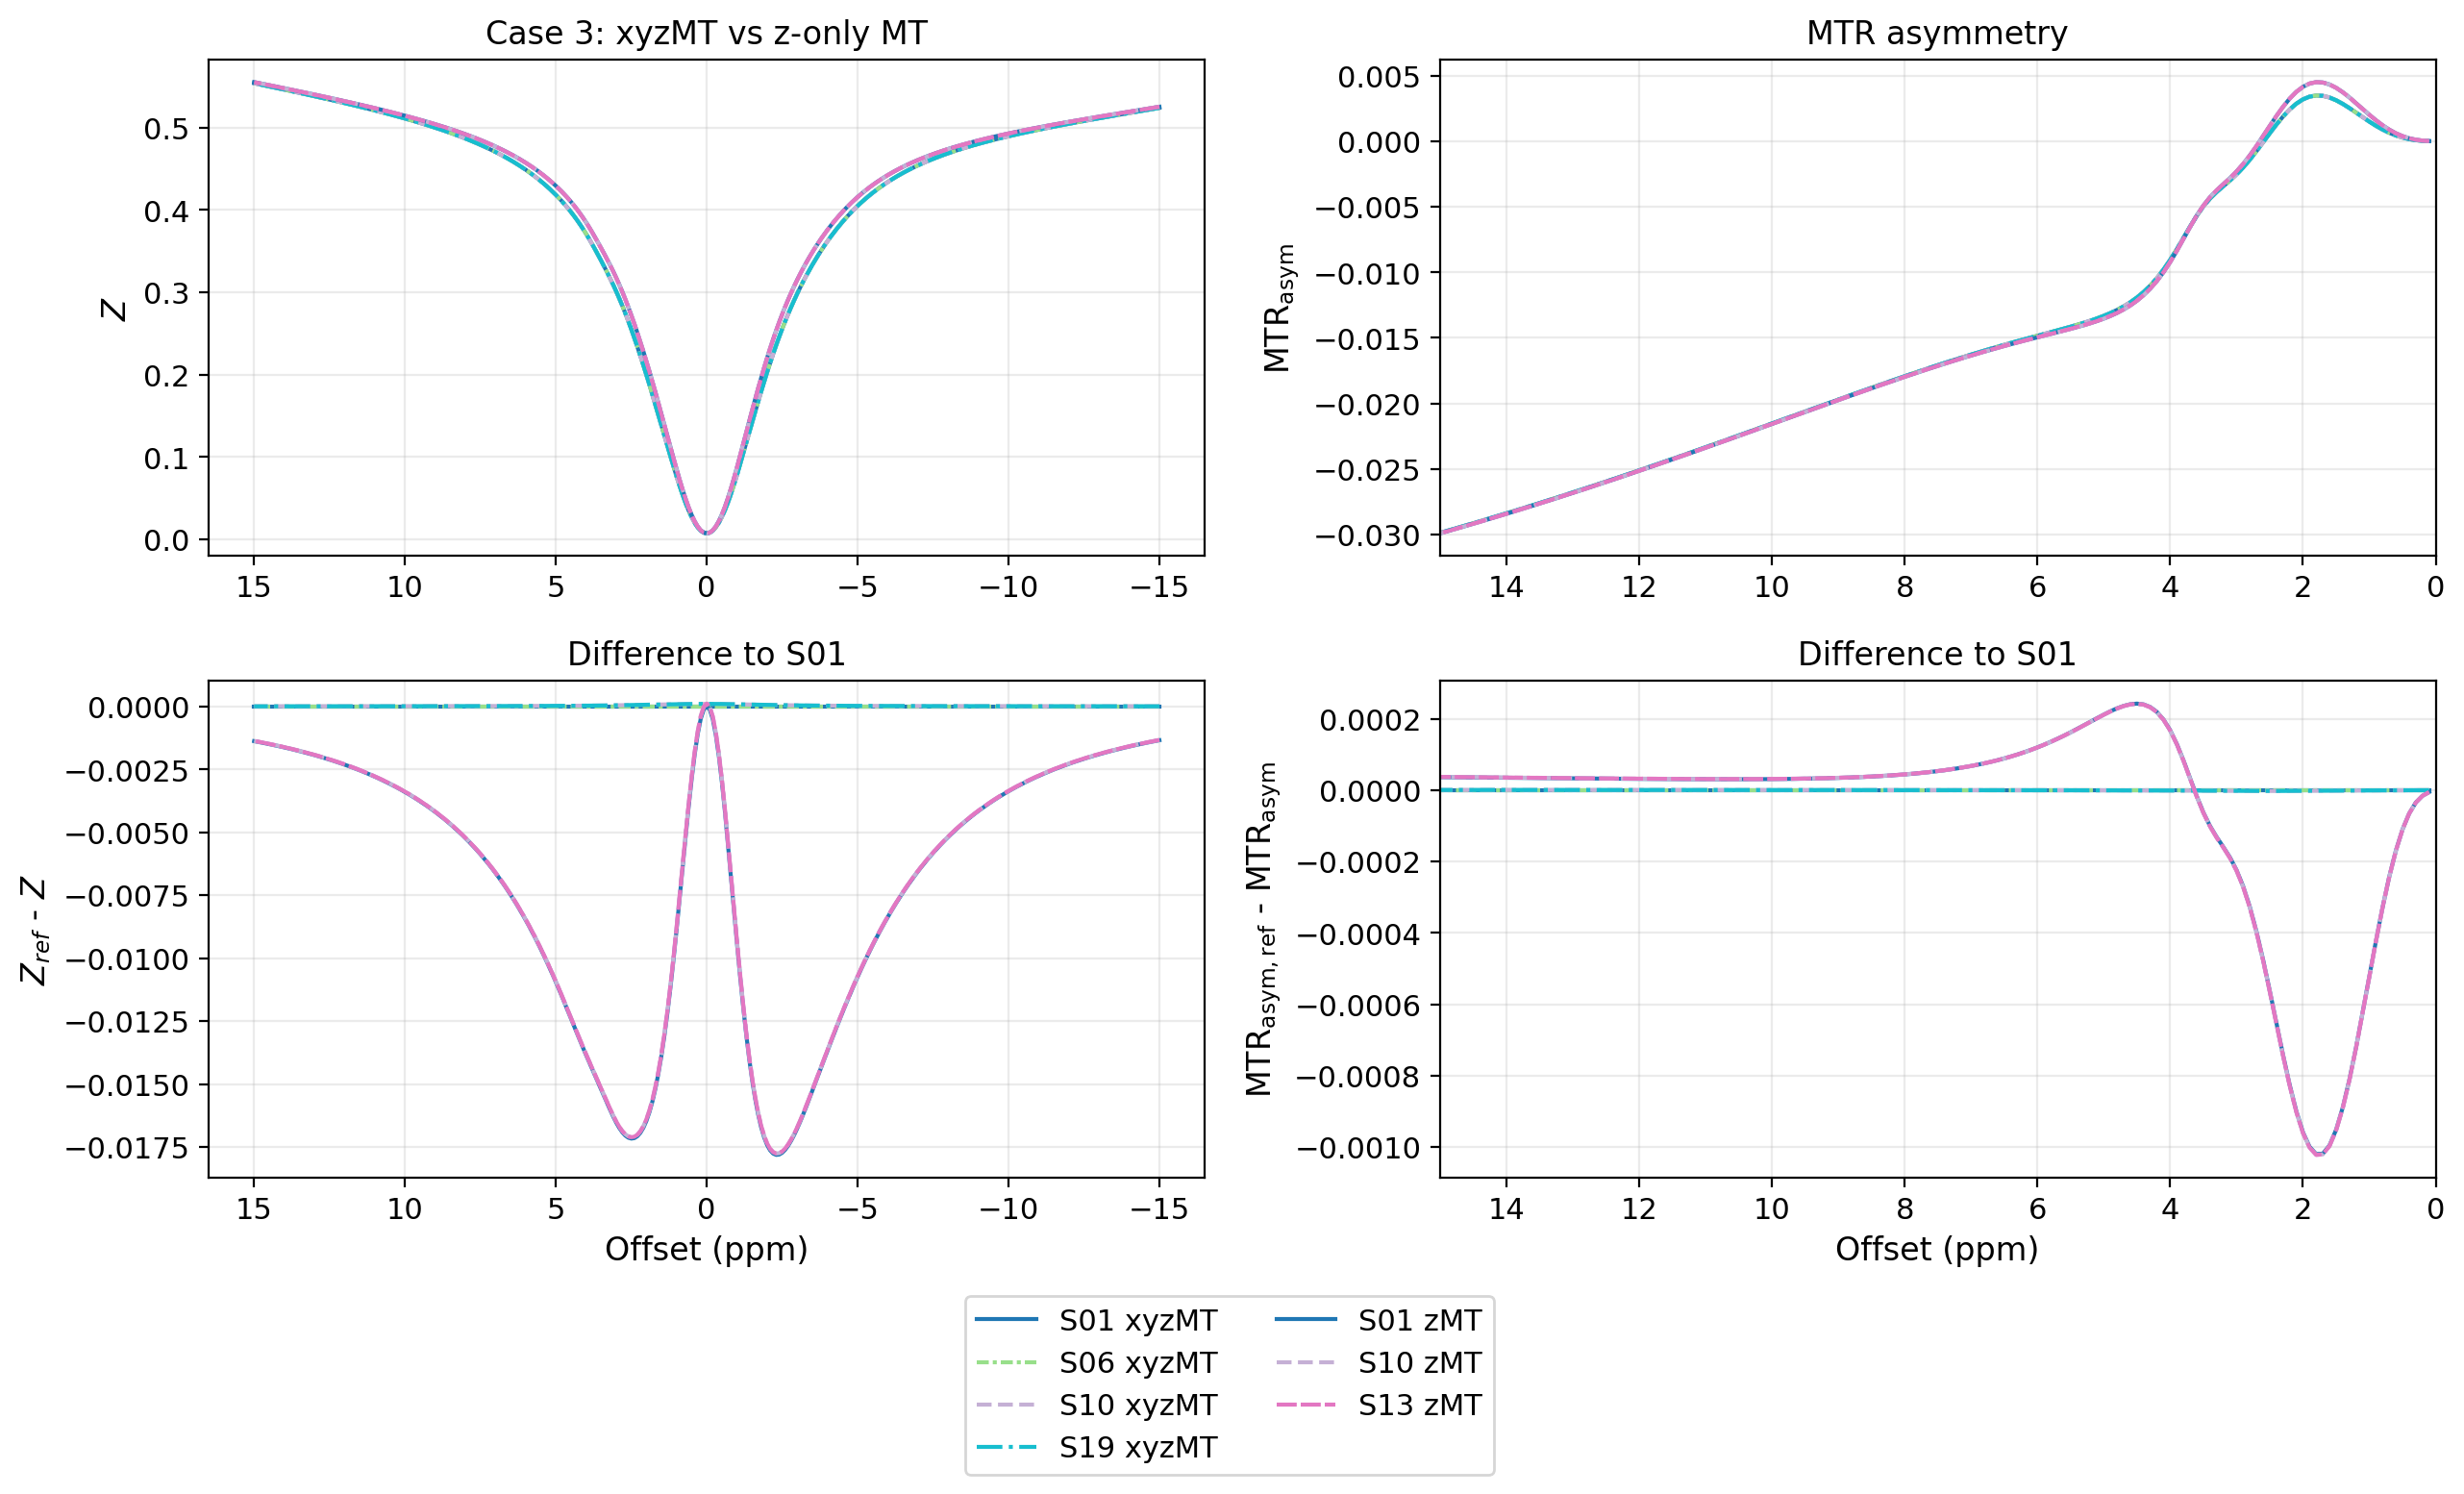
\includegraphics[width=1\linewidth]{figures/Case_3_zMT_comparison.png}
\caption{Selected entries for Case 3 showing full $M_{xyz}$ MT simulations (S01, S06, S10 and S19) in comparison with $z$-only MT simulations (S01, S10 and S13). The $M_{xyz}$ entries closely match with the chosen reference (here S01 xyzMT). The $z$-only MT entries show a significant difference to the reference, with close agreement between each other.}
\label{fig:ReasultszMT3}
\end{figure}

\begin{figure}[t]
\centering
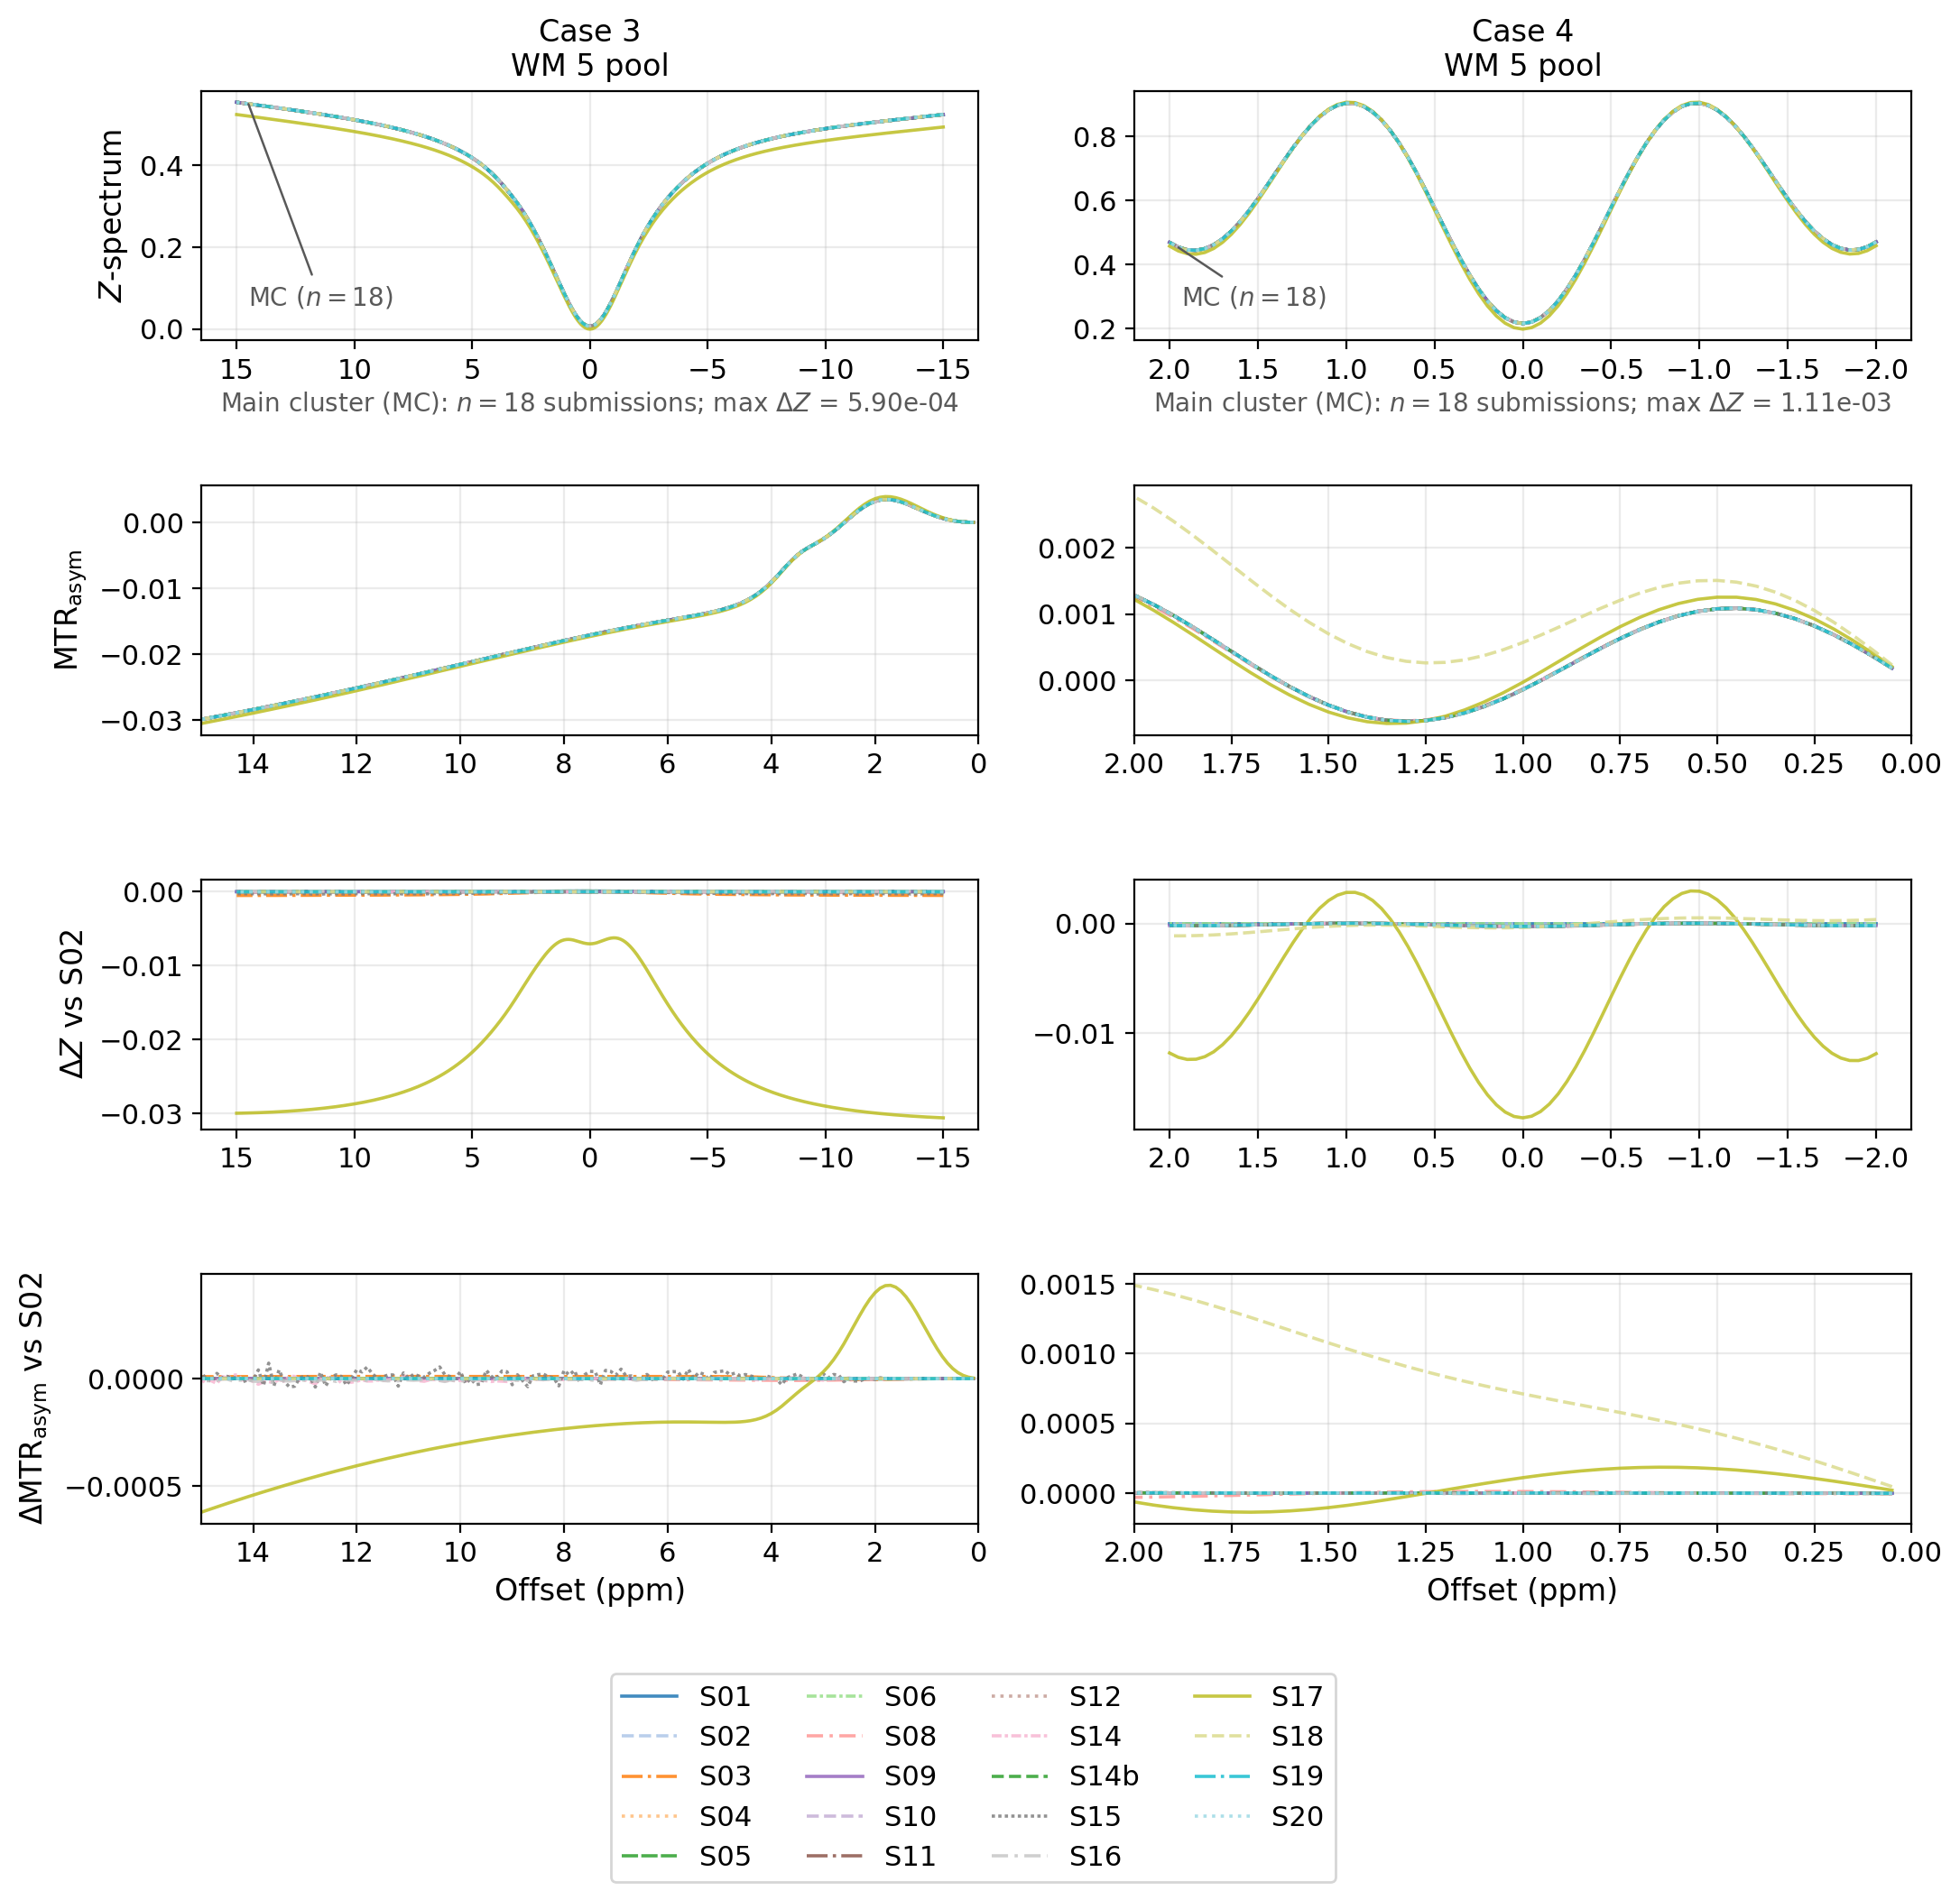
\includegraphics[width=1\linewidth]{figures/Figure_CASE_34.png}
\caption{Cases 3 and 4: simulated $Z$- and $MTR_{asym}$ spectra with differences to S02. The main cluster is marked in the Z-spectra plots and contained 18 (of 19) entries in Case 3 and 18 (of 19) entries in Case 4, with maximum deviations of $5.90\cdot10^{-04}$ and $1.11\cdot10^{-03}$, respectively within those clusters. S17 shows the largest deviations in both cases; in Case 4, S18 also differs noticeably in $MTR_{asym}$.}
\label{fig:ReasulsAll34}
\end{figure}


\begin{figure}[t]
\centering
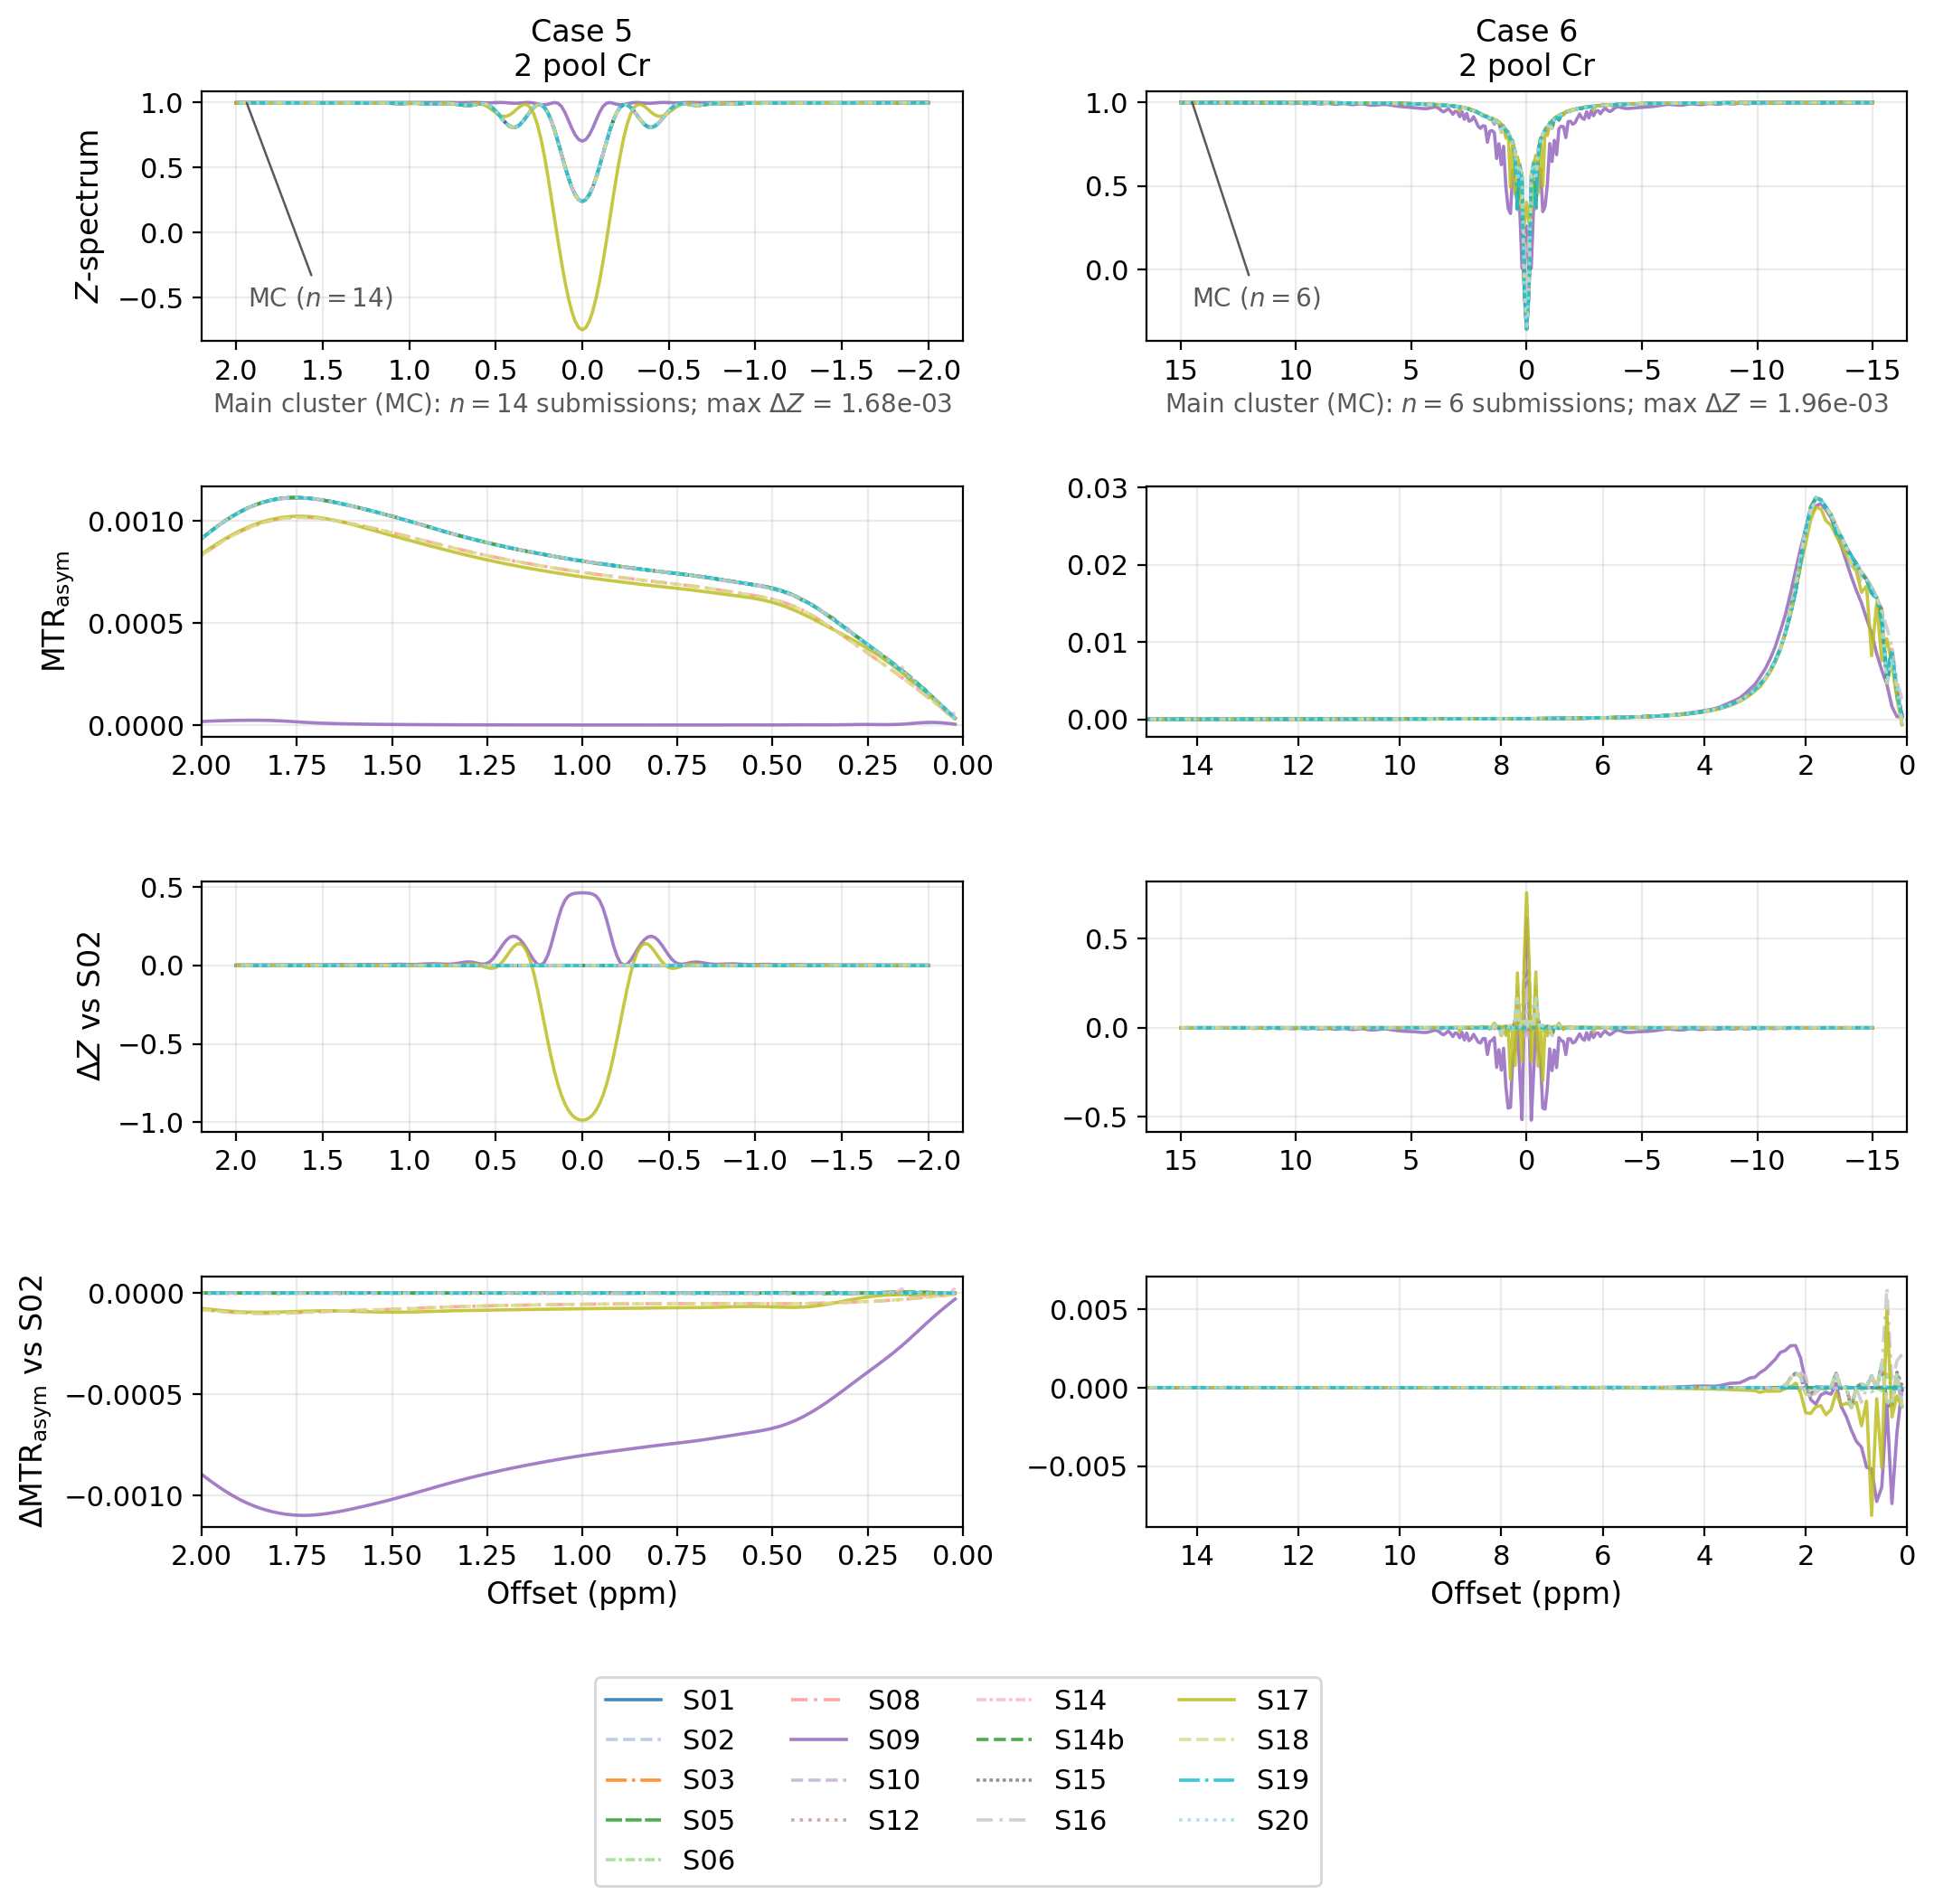
\includegraphics[width=1\linewidth]{figures/Figure_CASE_56.png}
\caption{Cases 5 and 6: simulated $Z$- and $MTR_{asym}$ spectra with differences to S02. The main cluster is marked in the Z-spectra plots and contained 14 (of 16) entries in Case 5 and 6 (of 17) entries in Case 6, with maximum deviations of $1.68\cdot10^{-03}$ and $1.96\cdot10^{-03}$, respectively within those clusters. S09 and S17 show the largest deviations in Case 5.}
\label{fig:ReasulsAll56}
\end{figure}

\begin{figure}[t]
\centering
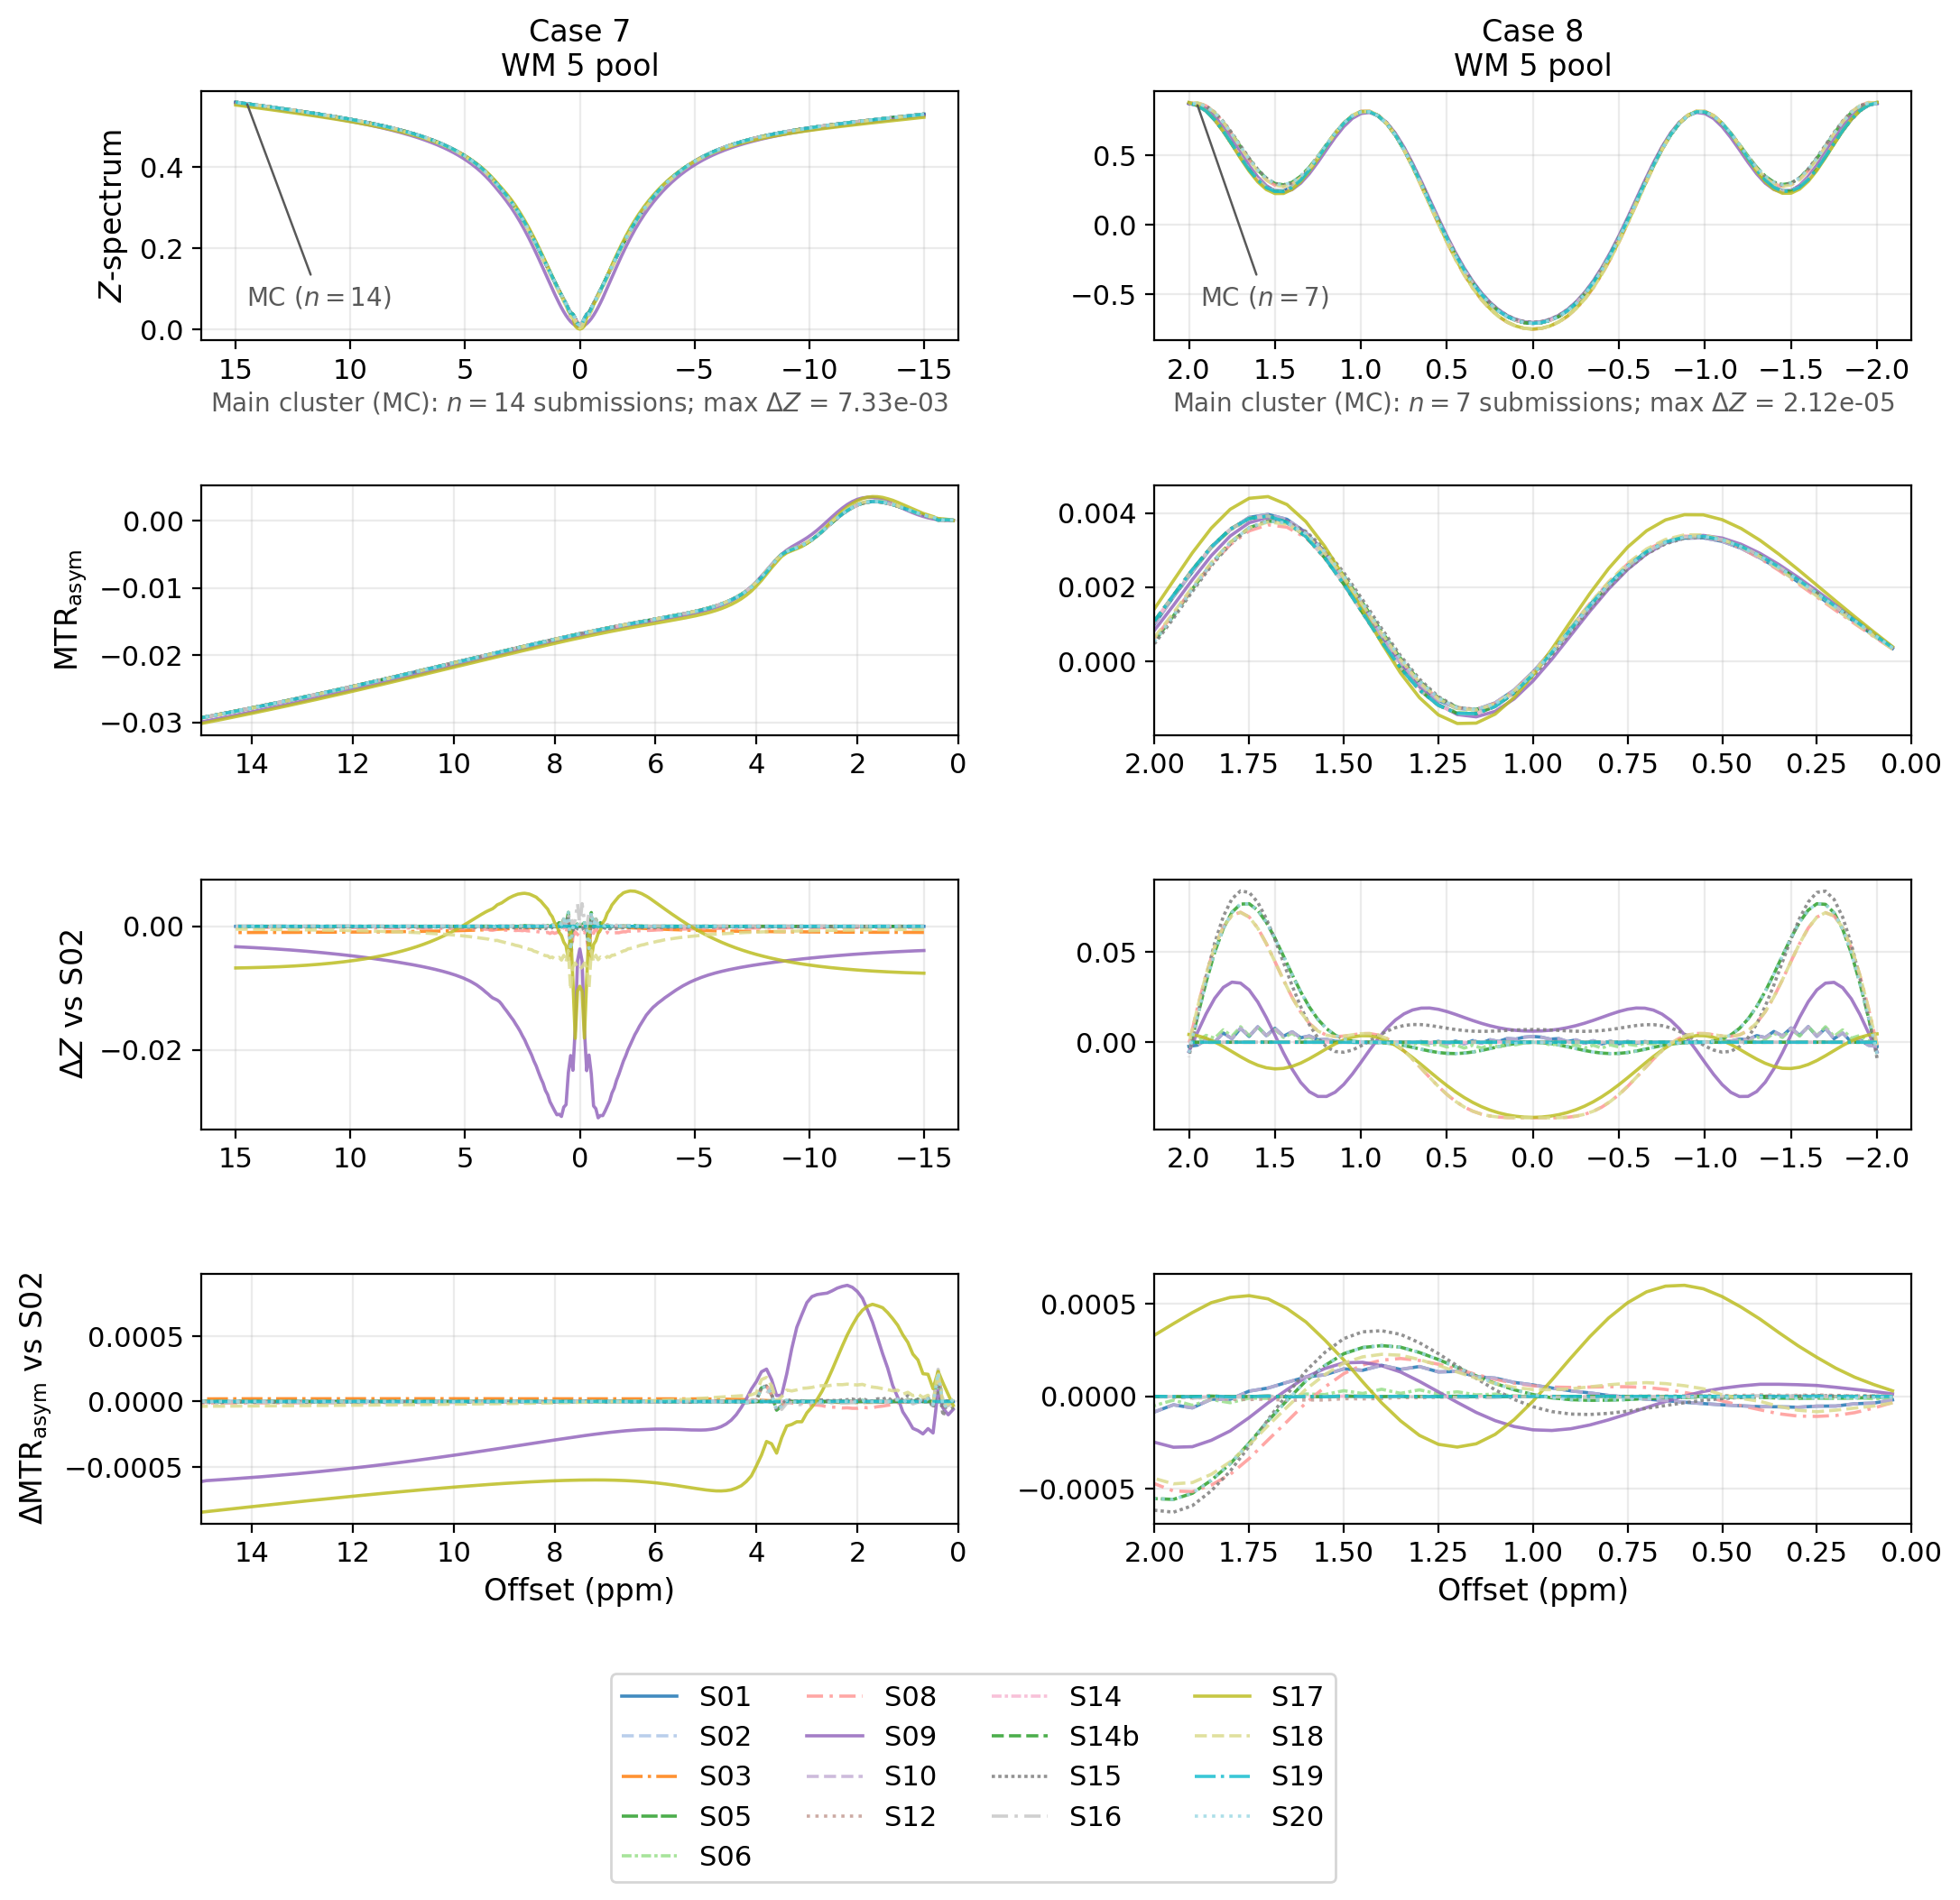
\includegraphics[width=1\linewidth]{figures/Figure_CASE_78.png}
\caption{Cases 7 and 8: simulated $Z$- and $MTR_{asym}$ spectra with differences to S02. The main cluster is marked in the Z-spectra plots and contained 14 (of 17) entries in Case 7 and 7 (of 17) entries in Case 8, with maximum deviations of $7.33\cdot10^{-03}$ and $2.12\cdot10^{-05}$, respectively within those clusters. In Case 7, S09, S18, and S19 deviate most strongly; Case 8 shows broader spread with several separated traces.}
\label{fig:ReasulsAll78}
\end{figure}

\begin{figure}[t]
\centering
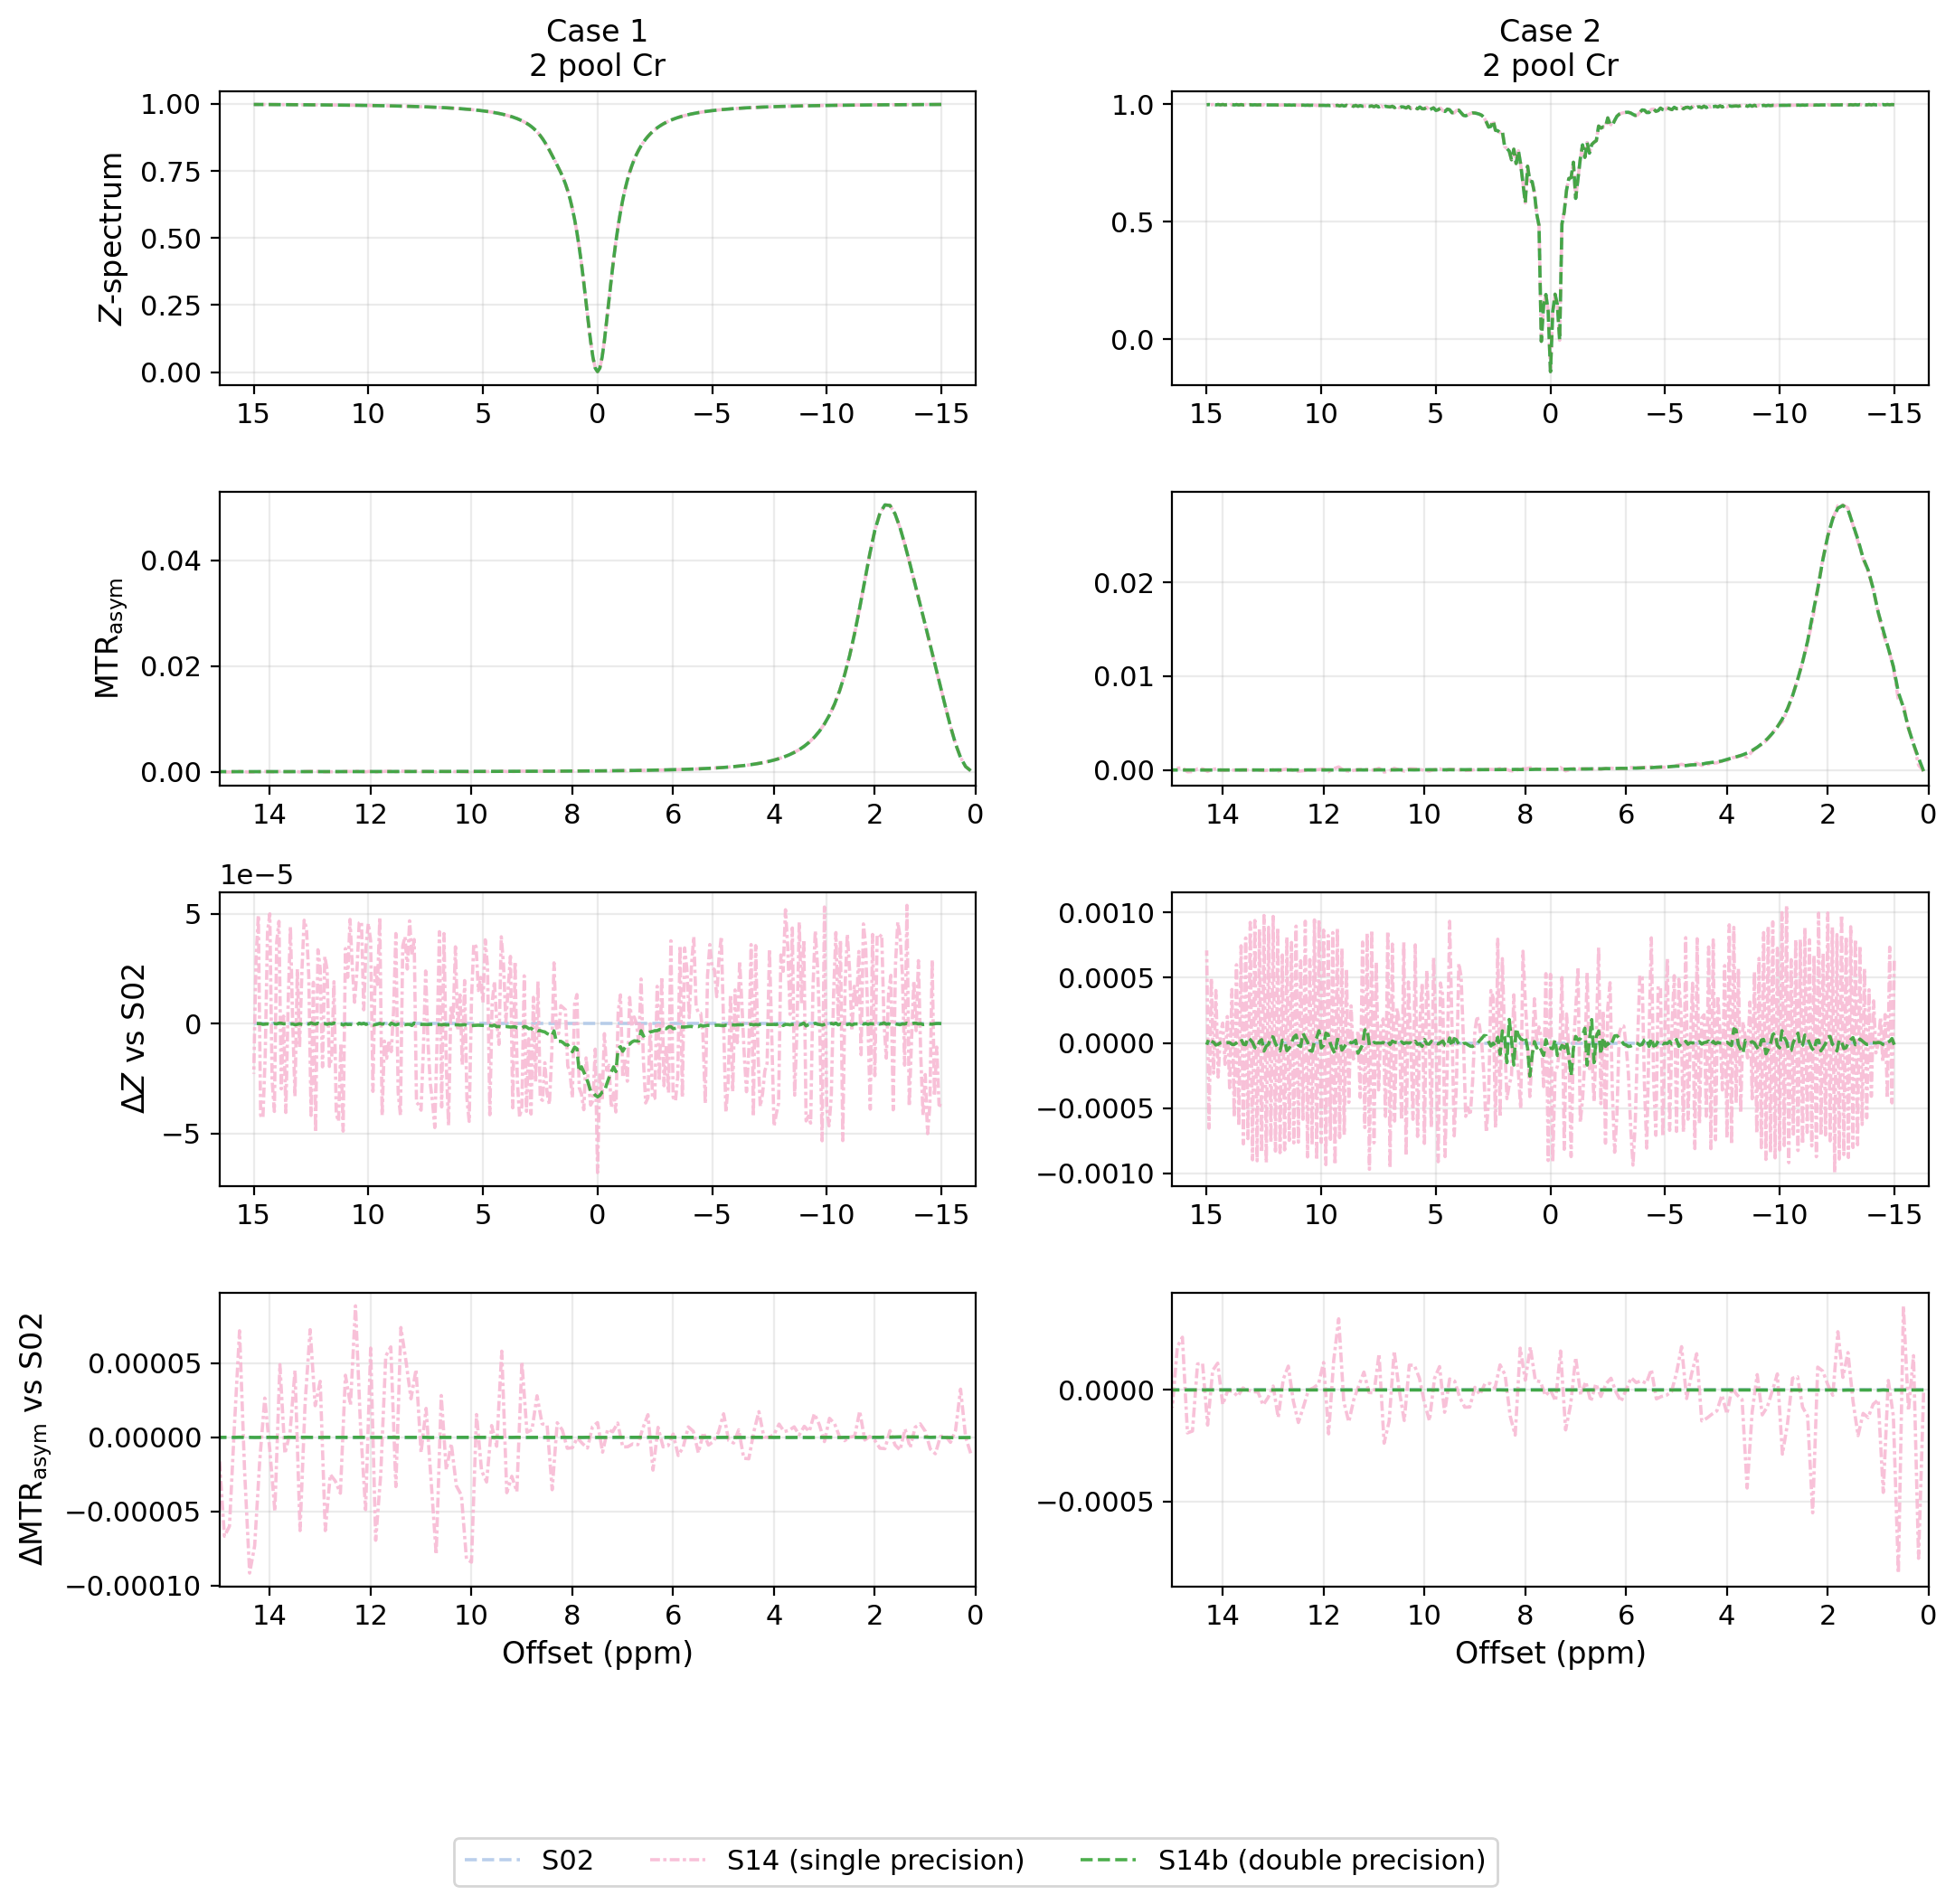
\includegraphics[width=1\linewidth]{figures/Figure_BART_precision_12.png}
\caption{Single- and double-precision BART simulations (S14 and S14b) compared with the reference S02 for Cases 1 and 2. In single precision high-frequency numerical noise is visible that is largely absent in the double-precision variant.}
\label{fig:BARTprecision}
\end{figure}

\begin{figure}[t]
\centering
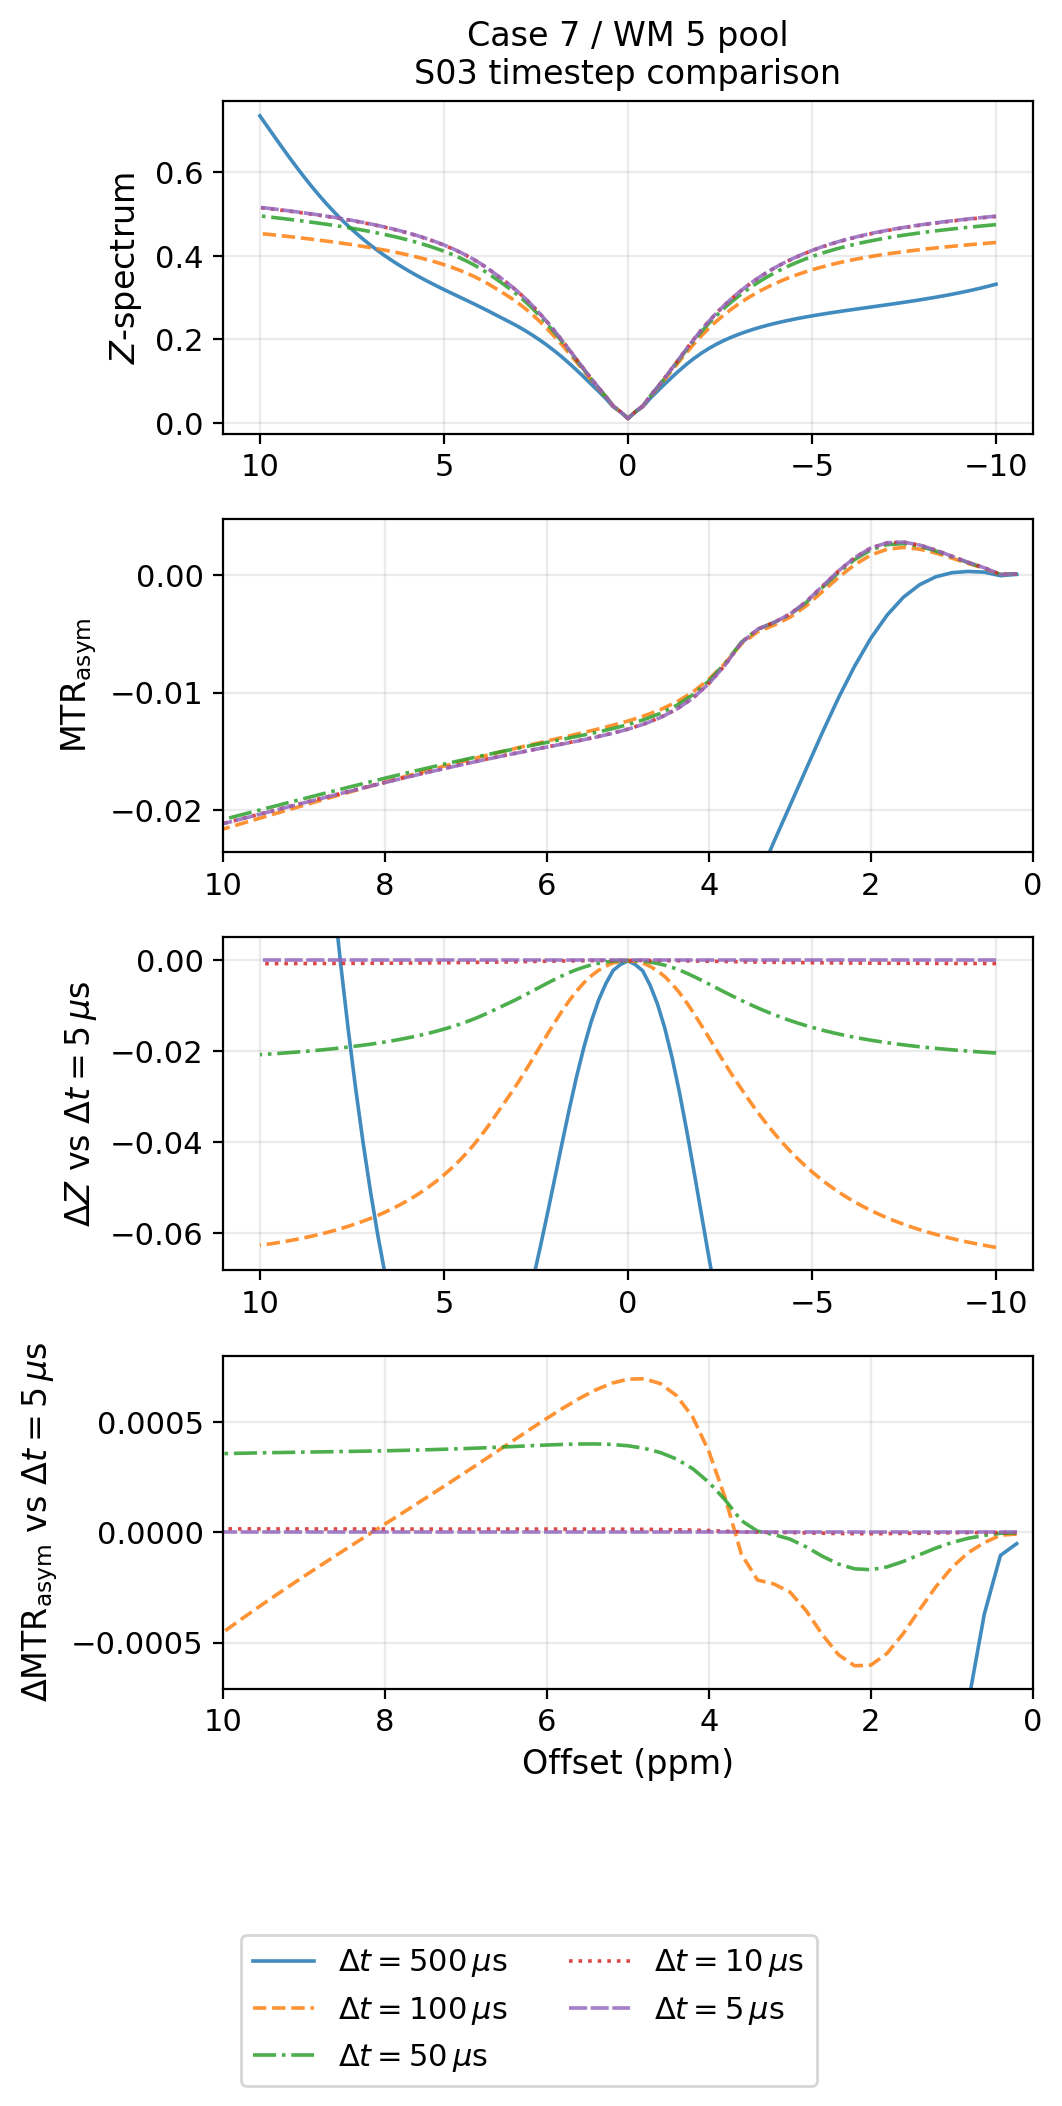
\includegraphics[width=0.5\linewidth]{figures/Case_7_timestep.png}
\caption{Case~7 $Z$- and $MTR_{\mathrm{asym}}$ spectra for submission S03 simulated with fixed timesteps from 500 to 5~$\mu$s. The lower two panels show differences to the finest timestep (5~$\mu$s). Axis limits in the lower two panels were chosen to highlight agreement among the smaller timesteps.}
\label{fig:Case7timestep}
\end{figure}



\section{Discussion}\label{Diss}
In this study we showed that a main cluster of agreeing simulations could be found for each case, consisting of 16 entries in the CW case, and 6 groups in the pulsed CEST case, which tentatively allows us to formulate a consensus on simulations. 
However, this study also shows that Bloch-McConnell simulations are not automatically interchangeable across independent implementations, even when the nominal pool model, RF preparation pulse trains, offsets, and initialization conditions are specified. The degree of agreement depended strongly on the simulation case. The long CW 2-pool case showed close agreement, whereas shorter saturation, shaped pulses, pulse trains, and the 5-pool white-matter model all increased the observed variability. These findings indicate that benchmark cases need to include both simple reference scenarios and more clinically realistic preparations; agreement in a steady-state-like 2-pool case alone is not sufficient to validate a simulation framework for quantitative CEST applications.

The first round separated several sources of variability. Case 1 was intended as the simplest baseline and showed the smallest spread, suggesting that most implementations handle the basic Bloch-McConnell evolution, offset convention, and relaxation/exchange terms similarly under near steady-state conditions. 
The larger spread in Case 2 suggests that transient behavior is more sensitive to numerical and implementation choices. Since the pool model and RF amplitude were unchanged between Cases 1 and 2, these differences point to details such as matrix exponentiation, ODE integration tolerances, pulse/discretization conventions for CW irradiation, or the precise handling of delays. The lower spread in Case 1 may reflect that the long saturation approaches a common steady-state solution, whereas the shorter preparation in Case 2 preserves differences in transient evolution.

The 5-pool model introduced a second major source of variability. The comparison of full $M_{xyz}$ and $z$-only MT implementations showed that these approaches produce systematically different spectra and should not be mixed without explicit labeling. This is expected because a $z$-only semisolid pool model approximates the MT pool using longitudinal saturation and an absorption lineshape, whereas a full $M_{xyz}$ implementation evolves transverse components explicitly. Both approaches may be useful in specific contexts, but they are not equivalent for the benchmark cases used here. For this reason, $z$-only MT results were retained in the data source but excluded from the main figures. 
The lineshape of the ssMT effect is an open question in the field, with Lorentzian, super Lorentzian, Gaussian, and other lineshapes being used in different studies \cite{Asslnder2022}. Depending on the investigated tissue and the specific application, different lineshapes may be more appropriate. The present benchmark does not address this question, but it highlights that the choice of MT modeling can have a substantial impact on the simulated spectra and should be clearly specified in future studies.
Furthermore, these lineshapes are often implemented using numerical approximations, such as discretization of the lineshape or interpolation around pole locations.
This can introduce additional variability, and possibly errors if not implemented carefully. 

The second round showed that shaped RF preparations are another important source of disagreement. The single Gaussian pulse produced the largest absolute Z-spectrum spread, even though the pulse shape was provided in a machine-readable file. This suggests that providing the shape alone does not fully eliminate ambiguity: interpolation of the RF waveform, time discretization, conversion between peak and RMS $B_1$, treatment of phase, and the specific pulse integration can all affect the result.
The pulse-train cases further amplify these choices because small differences are repeated many times and multiple pulses necessitate accurate handling of phase evolution and relaxation during interpulse delays.
Ambiguities in the challenge definition of the pulse shape were also reported by several participants, including the exact $B_1$ scaling, the time discretization of the pulse, and the handling of phase in the pulse train case.
The multi-pool model in Case 7 shows much closer agreement, indicating that the differences are not caused by the multi-pool model itself, but by the shaped pulse implementation and the long $T_1$ and $T_2$ values of water for the 2-pool model.
The long relaxation times of water in the 2-pool model lead to a slow decay of the magnetization, which necessitates accurate simulation throughout the pulse train, as any small difference in the magnetization evolution can accumulate and lead to significant differences in the final spectrum.


\subsection{Solver choices and differences}
In general, the results show that the same solution can be reached with different numerical strategies, provided that the implementations are sufficiently accurate for the RF preparation and pool model. Closely agreeing submissions used different approaches, including matrix exponentiation, Pad\'e approximations, eigenvalue decompositions, ODE solvers, operator splitting, and state-transition matrices that combine aspects of matrix-exponential and ODE propagation. Thus, the solver class itself does not appear to determine the result uniquely. Instead, deviations are more likely caused by the details of how the solver is applied, such as time-step selection, waveform discretization, convergence criteria, and the handling of very short relaxation constants.

One important distinction is whether the simulation uses fixed or adaptive time steps. A fixed time-step implementation can be efficient and reproducible, but the chosen step size must be short enough to resolve the fastest dynamics in the system. This becomes particularly relevant for shaped pulses and for full $M_{xyz}$ MT implementations, where very short $T_2$ values lead to rapidly decaying transverse components. If these dynamics are under-resolved, the resulting spectrum can deviate even when the pool parameters are nominally identical. Conversely, very small fixed time steps may increase memory use and computation time, especially for long pulse trains and many offsets.

Adaptive ODE solvers and matrix-exponential approaches avoid some of these limitations, but introduce their own implementation choices. ODE solvers depend on tolerances, step sizes, and event discretization. Matrix-exponential approaches depend on how the RF waveform is divided into constant-amplitude intervals and how the exponential is evaluated, for example by Pad\'e approximation or eigenvalue decomposition. For well-conditioned problems and carefully implemented solver choices these approaches should converge to the same solution, but differences can appear for long transient solutions with slow decays, when the RF pulse is coarsely sampled, when the ODE becomes stiff due to very short decay times, or approximations are used without convergence checks.

Figure~\ref{fig:BARTprecision} illustrates the impact of floating point precision
for the BART implementation.
In Case~2 (CW transient saturation), single-precision arithmetic introduced visible high-frequency noise in the difference spectra, whereas the double-precision variant reduced the peak numerical error by approximately a factor of four and the mean point-wise error by more than an order of magnitude. 
This indicates that floating-point precision can affect even CW CEST simulations when transient evolution is resolved over many integration steps.
While only shown here for BART, this is expected to affect all solver classes.
Nevertheless, the single-precision result still were precise enough
for practical applications in all examples.

Figure~\ref{fig:Case7timestep} shows a related effect in Case~7 for fixed-step operator-splitting timescale in S03: an overly coarse timestep of 500~$\mu$s produced a clearly incorrect spectrum, while progressively smaller timesteps converged toward the same solution. These findings support the view that solver accuracy must be validated for the specific RF preparation and exact numerical settings are important to achieve reproducible results.

The benchmark therefore suggests that future simulation reports should describe not only the mathematical model, but also the numerical propagation strategy. In particular, time-step strategy, RF resampling, solver tolerances or matrix-exponential method, and convergence checks should be documented to allow a more detailed comparison of simulation results.

\subsection{Implications for qMRI and future Bloch-McConnell simulations}
The relationship between Z-spectrum spread and $MTR_{\mathrm{asym}}$ spread was case dependent. In some cases, large Z-spectrum differences produced comparatively small $MTR_{\mathrm{asym}}$ differences, consistent with approximately symmetric deviations.
In other cases, especially when the 5-pool model was combined with pulsed saturation, differences became strongly asymmetric and led to larger $MTR_{\mathrm{asym}}$ variability. This is important for qCEST because many downstream analyses use asymmetry or fitted pool parameters rather than the raw Z-spectrum. A deviation that appears modest in Z can therefore still be relevant if it affects the spectral asymmetry near the fitted pool resonance.

The present comparison does not yet assign all deviations to a single cause. Several factors can interact, including RF definitions, MT-pool formulation, solver choice, implementation and accuracy, and waveform discretization. In addition, some differences arose from ambiguity in the original challenge description rather than from an error in a particular simulation package. The benchmark therefore serves two purposes: it identifies cases where implementations diverge, and it tested which parts of the simulation specification need to be stated for reproducible quantitative CEST.

A practical implication is that future CEST simulation studies should report implementation details that are often omitted, including whether MT pools are modeled as full $M_{xyz}$ or $z$-only systems, how shaped RF pulses are discretized and scaled, how phase evolution between pulses is treated, and how magnetization is initialized between offsets. The challenge repository has already been updated to clarify several of these points (\url{https://github.com/pulseq-cest/BMsim_challenge}). Continued use of shared machine-readable definitions, together with reference results and open analysis scripts, should make it possible to distinguish model choices from unintended implementation differences.

As a reference simulation we suggest the BMCTool results (S02) \cite{SchuenkeBMC}, which showed no significant deviation from the main cluster of results. The tool is easy to use with its Python interface and support for pulseq files. Therefore, comparing against BMCTool provides a quick and easy check for reasonable results, with small deviations being possible due to the above-mentioned implementation details. 


\section{Conclusion}\label{Conc}
This benchmark shows that independent Bloch-McConnell simulation frameworks can agree closely for simple reference cases, but may diverge substantially for transient saturation, shaped RF pulses, pulse trains, and multi-pool models with MT. Clear specification of MT modeling, RF power definitions, pulse discretization, and initialization conditions is therefore essential for reproducible quantitative CEST. For newly implemented simulations we suggest comparing against the BMCTool results (S02). The provided open challenge data and analysis scripts provide a basis for continued community validation and for developing more standardized CEST simulation practice. 

% This is a seperate field in the online submission form, but we include it here for completeness.
% \subsection*{Data Availability Statement}
% The benchmark specifications, pool-model definitions, and sequence files are available in the public GitHub repository at \url{https://github.com/pulseq-cest/BMsim_challenge}. The Python analysis scripts used to parse the results, compute summary metrics, and generate the manuscript figures are available in the same repository in the scripts folder. Pool-model parameters and additional submission descriptions are provided in the Supporting Information document. During the study, submitted Z-spectra were collected in a shared Google spreadsheet: (\url{https://docs.google.com/spreadsheets/d/1JN7VN-f1ktDrJgokb0FlUFwkH0MWYlPA_jSfnQoFOVc}). 
% While the spreadsheet might still be updated the dataset used to generate the figures and analyses in this manuscript is archived at \url{https://doi.org/10.5281/zenodo.21265597}.

\subsection*{Author contributions}

M.Z. and P.S. designed the study. M.Z., and P.S. defined the simulation cases and specifications. M.Z., P.S. and M.H coordinated the study and collected results. M.H. performed the analysis and wrote the initial paper draft. All named authors submitted their results and contributed to writing, editing and reviewing of the manuscript.

\subsection*{Acknowledgements}

The authors thank all participating groups for contributing simulation results to the benchmark. AI-assisted coding tools were used to develop and refine the Python analysis scripts for parsing submitted results, computing summary metrics, and generating manuscript figures. AI-assisted writing tools were also used to support drafting and editing of the manuscript text. All authors reviewed, edited, and approved the final content and take responsibility for the published work.
This research was funded in whole or in part by the Austrian Science Fund (FWF) 10.55776/F100800 and 10.55776/I4870. This work was partially supported by Deutsche Forschungsgemeinschaft (DFG, German Research Foundation) grants 372486779 (SFB1340) and ZA 814/15-1.
\bibliographystyle{MRM-AMA}
\bibliography{MRM-AMA}%
\vfill\pagebreak

\end{document}
